% Options for packages loaded elsewhere
\PassOptionsToPackage{unicode}{hyperref}
\PassOptionsToPackage{hyphens}{url}
\PassOptionsToPackage{dvipsnames,svgnames,x11names}{xcolor}
\documentclass[
  brazilian,
  a4paper,12pt,oneside]{report}
\usepackage{xcolor}
\usepackage[margin=2.5cm]{geometry}
\usepackage{amsmath,amssymb}
\setcounter{secnumdepth}{-\maxdimen} % remove section numbering
\usepackage{iftex}
\ifPDFTeX
  \usepackage[T1]{fontenc}
  \usepackage[utf8]{inputenc}
  \usepackage{textcomp} % provide euro and other symbols
\else % if luatex or xetex
  \usepackage{unicode-math} % this also loads fontspec
  \defaultfontfeatures{Scale=MatchLowercase}
  \defaultfontfeatures[\rmfamily]{Ligatures=TeX,Scale=1}
\fi
\usepackage{lmodern}
\ifPDFTeX\else
  % xetex/luatex font selection
\fi
% Use upquote if available, for straight quotes in verbatim environments
\IfFileExists{upquote.sty}{\usepackage{upquote}}{}
\IfFileExists{microtype.sty}{% use microtype if available
  \usepackage[]{microtype}
  \UseMicrotypeSet[protrusion]{basicmath} % disable protrusion for tt fonts
}{}
\makeatletter
\@ifundefined{KOMAClassName}{% if non-KOMA class
  \IfFileExists{parskip.sty}{%
    \usepackage{parskip}
  }{% else
    \setlength{\parindent}{0pt}
    \setlength{\parskip}{6pt plus 2pt minus 1pt}}
}{% if KOMA class
  \KOMAoptions{parskip=half}}
\makeatother
\usepackage{longtable,booktabs,array}
\newcounter{none} % for unnumbered tables
\usepackage{calc} % for calculating minipage widths
% Correct order of tables after \paragraph or \subparagraph
\usepackage{etoolbox}
\makeatletter
\patchcmd\longtable{\par}{\if@noskipsec\mbox{}\fi\par}{}{}
\makeatother
% Allow footnotes in longtable head/foot
\IfFileExists{footnotehyper.sty}{\usepackage{footnotehyper}}{\usepackage{footnote}}
\makesavenoteenv{longtable}
\usepackage{graphicx}
\makeatletter
\newsavebox\pandoc@box
\newcommand*\pandocbounded[1]{% scales image to fit in text height/width
  \sbox\pandoc@box{#1}%
  \Gscale@div\@tempa{\textheight}{\dimexpr\ht\pandoc@box+\dp\pandoc@box\relax}%
  \Gscale@div\@tempb{\linewidth}{\wd\pandoc@box}%
  \ifdim\@tempb\p@<\@tempa\p@\let\@tempa\@tempb\fi% select the smaller of both
  \ifdim\@tempa\p@<\p@\scalebox{\@tempa}{\usebox\pandoc@box}%
  \else\usebox{\pandoc@box}%
  \fi%
}
% Set default figure placement to htbp
\def\fps@figure{htbp}
\makeatother
\ifLuaTeX
\usepackage[bidi=basic,shorthands=off]{babel}
\else
\usepackage[bidi=default,shorthands=off]{babel}
\fi
\ifLuaTeX
  \usepackage{selnolig} % disable illegal ligatures
\fi
\setlength{\emergencystretch}{3em} % prevent overfull lines
\providecommand{\tightlist}{%
  \setlength{\itemsep}{0pt}\setlength{\parskip}{0pt}}
\usepackage{bookmark}
\IfFileExists{xurl.sty}{\usepackage{xurl}}{} % add URL line breaks if available
\urlstyle{same}
\hypersetup{
  pdftitle={Manual do Usuário},
  pdfauthor={Documentação do sistema AGIA},
  pdflang={pt-BR},
  colorlinks=true,
  linkcolor={blue},
  filecolor={Maroon},
  citecolor={Blue},
  urlcolor={blue},
  pdfcreator={LaTeX via pandoc}}

\title{Manual do Usuário}
\usepackage{etoolbox}
\makeatletter
\providecommand{\subtitle}[1]{% add subtitle to \maketitle
  \apptocmd{\@title}{\par {\large #1 \par}}{}{}
}
\makeatother
\subtitle{Sistema AGIA --- Prospecção Tecnológica}
\author{Documentação do sistema AGIA}
\date{17/10/2026}

\begin{document}
\maketitle

{
\setcounter{tocdepth}{1}
\tableofcontents
}
\emph{Atualizado em 17/10/2026.}

O AGIA apoia a \textbf{prospecção tecnológica}. A partir de um tema de
pesquisa, o sistema busca patentes e artigos científicos, extrai os
termos mais relevantes, analisa o cenário (depositantes, instituições,
classificações e evolução no tempo) e monta um \textbf{relatório técnico
no padrão REPTEC/AGITEC}, em LaTeX e PDF.

Antes de usar, o sistema precisa estar instalado e em execução, e o
administrador precisa ter configurado as credenciais das bases de busca.
A seção de configurações deste manual explica o que o administrador pode
ajustar.

\begin{quote}
\textbf{Sobre as capturas de tela:} as imagens deste manual foram feitas
em uma versão de desenvolvimento da interface. Alguns rótulos podem ter
mudado depois. Quando houver diferença relevante, o texto indica o
rótulo atual.
\end{quote}

\begin{center}\rule{0.5\linewidth}{0.5pt}\end{center}

\chapter{1. Conceitos básicos}\label{conceitos-buxe1sicos}

{\def\LTcaptype{none} % do not increment counter
\begin{longtable}[]{@{}
  >{\raggedright\arraybackslash}p{(\linewidth - 2\tabcolsep) * \real{0.3333}}
  >{\raggedright\arraybackslash}p{(\linewidth - 2\tabcolsep) * \real{0.6667}}@{}}
\toprule\noalign{}
\begin{minipage}[b]{\linewidth}\raggedright
Termo
\end{minipage} & \begin{minipage}[b]{\linewidth}\raggedright
Significado
\end{minipage} \\
\midrule\noalign{}
\endhead
\bottomrule\noalign{}
\endlastfoot
\textbf{Sessão} (ou \textbf{prospecção}) & Uma pesquisa completa, do
tema ao relatório. Cada sessão pode ser salva e retomada. \\
\textbf{Tema} & O assunto da prospecção. É o único campo obrigatório. \\
\textbf{Refinamento} & Variações mais específicas do tema, sugeridas
pela IA. \\
\textbf{Query} & A expressão de busca enviada às bases. Há uma query
\textbf{exploratória} (restrita, para conhecer o campo) e uma
\textbf{final} (mais ampla). \\
\textbf{Busca exploratória} & Uma amostra pequena, usada para entender o
campo e descobrir termos. \\
\textbf{Busca final} & A busca completa. Seus resultados alimentam as
análises, os gráficos e o relatório. \\
\textbf{Termos} & Palavras e expressões extraídas automaticamente dos
títulos e resumos encontrados. \\
\textbf{Patentes} & Documentos de patente, das bases OPS (Escritório
Europeu de Patentes) ou Lens. \\
\textbf{Artigos} & Publicações científicas, das bases Scopus ou Lens. \\
\textbf{Curva S} & Gráfico da evolução cumulativa de documentos no
tempo, com um modelo de ciclo de vida. \\
\textbf{Tokens} & Unidades de texto processadas pela IA. A tela de Busca
mostra quantos a sessão consumiu. \\
\textbf{REPTEC/AGITEC} & Modelo de relatório técnico usado como
referência pelo sistema. \\
\end{longtable}
}

\begin{center}\rule{0.5\linewidth}{0.5pt}\end{center}

\chapter{2. Navegação}\label{navegauxe7uxe3o}

\section{2.1 Barra lateral}\label{barra-lateral}

O menu à esquerda dá acesso às telas principais. Ele pode ser recolhido
com a seta no topo, deixando só os ícones (com dicas ao passar o mouse).

{\def\LTcaptype{none} % do not increment counter
\begin{longtable}[]{@{}
  >{\raggedright\arraybackslash}p{(\linewidth - 4\tabcolsep) * \real{0.2833}}
  >{\raggedright\arraybackslash}p{(\linewidth - 4\tabcolsep) * \real{0.1333}}
  >{\raggedright\arraybackslash}p{(\linewidth - 4\tabcolsep) * \real{0.5833}}@{}}
\toprule\noalign{}
\begin{minipage}[b]{\linewidth}\raggedright
Item
\end{minipage} & \begin{minipage}[b]{\linewidth}\raggedright
Tela
\end{minipage} & \begin{minipage}[b]{\linewidth}\raggedright
Para que serve
\end{minipage} \\
\midrule\noalign{}
\endhead
\bottomrule\noalign{}
\endlastfoot
\textbf{Start} (ícone de energia) & Prospecção & Criar e conduzir uma
nova prospecção, nas quatro etapas. \\
\textbf{Settings} (engrenagem) & Configurações & Ajustar parâmetros do
sistema. \\
\textbf{Statistics} (gráfico) & Estatísticas & Visão geral de todas as
prospecções. \\
\textbf{Search} (lupa) & Busca & Listar, retomar e abrir relatórios das
sessões salvas. \\
\end{longtable}
}

No canto superior direito ficam o menu \textbf{Documentação}, que reúne
o guia do usuário, a referência da API e as perguntas frequentes dentro
do próprio sistema, o link \textbf{Sobre} e a versão do sistema.

\begin{quote}
\textbf{Durante uma prospecção, o menu fica bloqueado.} Isso evita
perder progresso não salvo por engano. Para sair, salve o progresso ou
conclua a sessão. O navegador também avisa antes de fechar a aba.
\end{quote}

\begin{quote}
\textbf{Rodapé da barra lateral:} em versões anteriores, mostrava
``LLM'' e ``API Artigos'' com valores fixos, que não refletiam a
configuração atual. Para saber qual IA e qual base estão em uso,
consulte a tela de Configurações.
\end{quote}

\section{2.2 Barra de etapas}\label{barra-de-etapas}

Durante a prospecção, uma barra no topo da tela mostra onde você está.
Ela tem quatro etapas principais, e cada uma tem subetapas:

{\def\LTcaptype{none} % do not increment counter
\begin{longtable}[]{@{}
  >{\raggedright\arraybackslash}p{(\linewidth - 4\tabcolsep) * \real{0.0508}}
  >{\raggedright\arraybackslash}p{(\linewidth - 4\tabcolsep) * \real{0.3390}}
  >{\raggedright\arraybackslash}p{(\linewidth - 4\tabcolsep) * \real{0.6102}}@{}}
\toprule\noalign{}
\begin{minipage}[b]{\linewidth}\raggedright
\#
\end{minipage} & \begin{minipage}[b]{\linewidth}\raggedright
Etapa
\end{minipage} & \begin{minipage}[b]{\linewidth}\raggedright
Subetapas
\end{minipage} \\
\midrule\noalign{}
\endhead
\bottomrule\noalign{}
\endlastfoot
1 & \textbf{Input Inicial} & Refinamento de Parâmetros \\
2 & \textbf{Exploração Inicial} & Resultados Iniciais · Amostragem de
Termos \\
3 & \textbf{Exploração Final} & Análise de Resultados · Criação de
Gráficos \\
4 & \textbf{Geração do Relatório} & --- \\
\end{longtable}
}

Etapas já concluídas aparecem preenchidas. A etapa atual fica destacada.

\begin{center}\rule{0.5\linewidth}{0.5pt}\end{center}

\chapter{3. Visão geral do fluxo}\label{visuxe3o-geral-do-fluxo}

\begin{verbatim}
Input Inicial --> Exploração Inicial --> Exploração Final --> Geração do Relatório
(tema e         (buscas exploratórias,   (busca final,        (metadados, seções,
 refinamento)    termos)                  análises, gráficos)  .tex, PDF)
\end{verbatim}

Em resumo:

\begin{enumerate}
\def\labelenumi{\arabic{enumi}.}
\tightlist
\item
  Você descreve o \textbf{tema} e, se quiser, pede à IA variações mais
  específicas.
\item
  O sistema faz uma \textbf{busca exploratória} em patentes e artigos.
  Você escolhe a query.
\item
  Dos resultados, o sistema extrai \textbf{termos}. Você escolhe quais
  usar.
\item
  Com esses termos, a IA monta a \textbf{query final}. Você revisa e
  confirma a busca final.
\item
  O sistema \textbf{analisa} os resultados e gera os \textbf{gráficos}.
\item
  Você preenche os \textbf{metadados} do relatório, gera o texto das
  \textbf{seções}, monta o documento LaTeX e, por fim, edita e compila o
  PDF.
\end{enumerate}

O tempo de cada etapa depende das bases consultadas, da quantidade de
documentos e do modelo de IA configurado. As etapas de busca e de
geração de texto são as mais lentas.

\begin{center}\rule{0.5\linewidth}{0.5pt}\end{center}

\chapter{4. Etapa 1 --- Parâmetros da
prospecção}\label{etapa-1-paruxe2metros-da-prospecuxe7uxe3o}

\section{4.1 Preenchendo o
formulário}\label{preenchendo-o-formuluxe1rio}

A tela \textbf{Parâmetros da Prospecção} pede os dados da pesquisa. Só o
\textbf{tema} é obrigatório para avançar ou salvar o progresso.

\begin{figure}
\centering
\pandocbounded{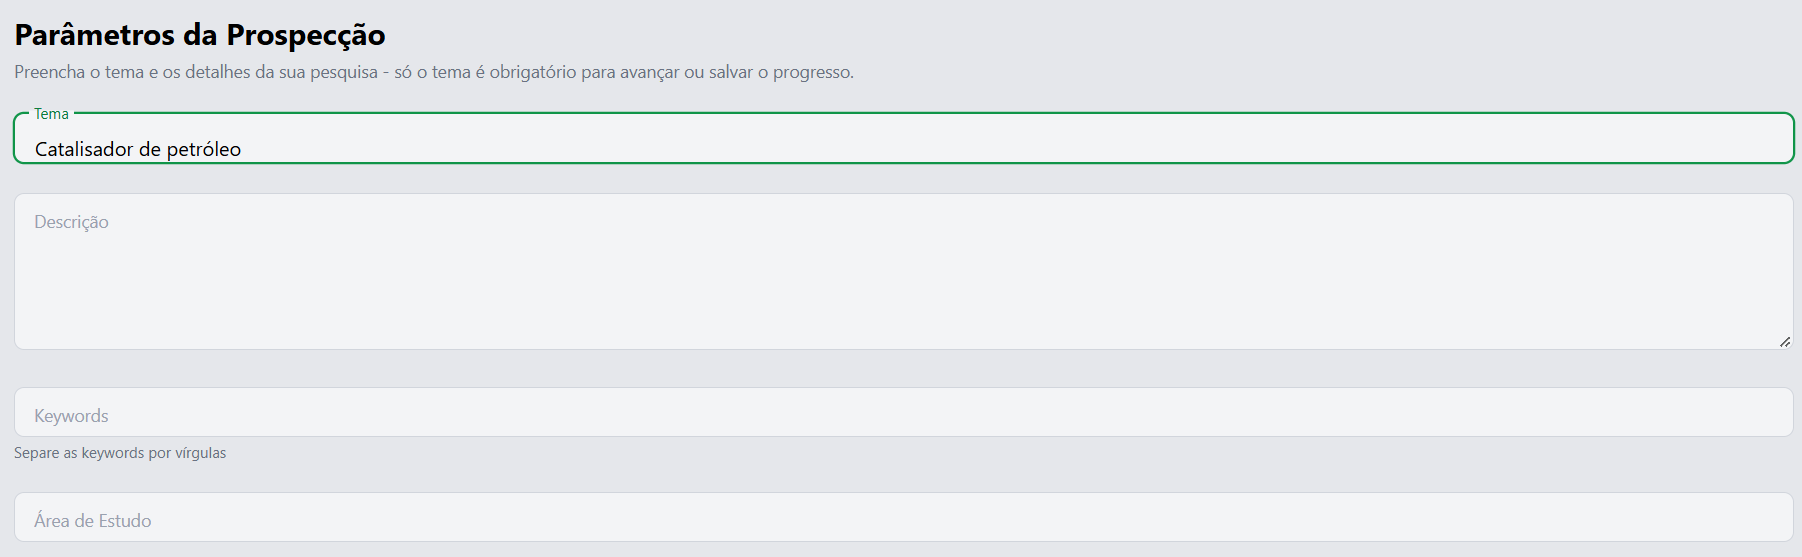
\includegraphics[keepaspectratio,alt={Formulário de parâmetros da prospecção preenchido com o tema ``Catalisador de petróleo''.}]{imagens/02-parametros.png}}
\caption{Formulário de parâmetros da prospecção preenchido com o tema
``Catalisador de petróleo''.}
\end{figure}

{\def\LTcaptype{none} % do not increment counter
\begin{longtable}[]{@{}
  >{\raggedright\arraybackslash}p{(\linewidth - 4\tabcolsep) * \real{0.2034}}
  >{\raggedright\arraybackslash}p{(\linewidth - 4\tabcolsep) * \real{0.1186}}
  >{\raggedright\arraybackslash}p{(\linewidth - 4\tabcolsep) * \real{0.6780}}@{}}
\toprule\noalign{}
\begin{minipage}[b]{\linewidth}\raggedright
Campo
\end{minipage} & \begin{minipage}[b]{\linewidth}\raggedright
Obrigatório
\end{minipage} & \begin{minipage}[b]{\linewidth}\raggedright
Como preencher
\end{minipage} \\
\midrule\noalign{}
\endhead
\bottomrule\noalign{}
\endlastfoot
\textbf{Tema} & Sim & O assunto principal. Ex.: ``baterias de estado
sólido'', ``inteligência artificial em saúde''. \\
\textbf{Descrição} & Não & Detalhes do projeto ou da área de interesse.
Quanto mais claro, melhor o refinamento. \\
\textbf{Keywords} & Não & Palavras-chave separadas por vírgulas. \\
\textbf{Área de Estudo} & Não & Campo de conhecimento. Ex.: ``Engenharia
de Materiais''. \\
\end{longtable}
}

Os botões do rodapé:

\begin{itemize}
\tightlist
\item
  \textbf{Refinar parâmetros} --- leva à subetapa de refinamento, onde a
  IA sugere variações do tema.
\item
  \textbf{Gerar Query} --- pula o refinamento e segue para a Exploração
  Inicial usando o tema exatamente como foi digitado.
\item
  \textbf{Avançar} --- próxima etapa, quando já existe resultado gerado
  para o que você preencheu.
\item
  \textbf{Cancelar} --- encerra a prospecção sem salvar e limpa o
  formulário. Uma sessão já salva continua na tela de Busca; o que não
  foi salvo é perdido.
\end{itemize}

O rótulo do botão muda conforme o que já foi gerado. Se aparecer
\textbf{Avançar} ou \textbf{Ver parâmetros} no lugar de \textbf{Gerar
Query} ou \textbf{Refinar parâmetros}, o sistema está reaproveitando o
resultado anterior, porque nada relevante mudou.

\begin{quote}
\textbf{Editar qualquer campo aqui invalida o que já foi refinado nas
etapas seguintes.} Isso é esperado: a IA precisa gerar de novo a partir
da entrada nova.
\end{quote}

\section{4.2 Refinamento de
parâmetros}\label{refinamento-de-paruxe2metros}

Ao clicar em \textbf{Refinar parâmetros}, a tela \textbf{Escolha qual
parâmetro utilizaremos} é aberta.

\begin{figure}
\centering
\pandocbounded{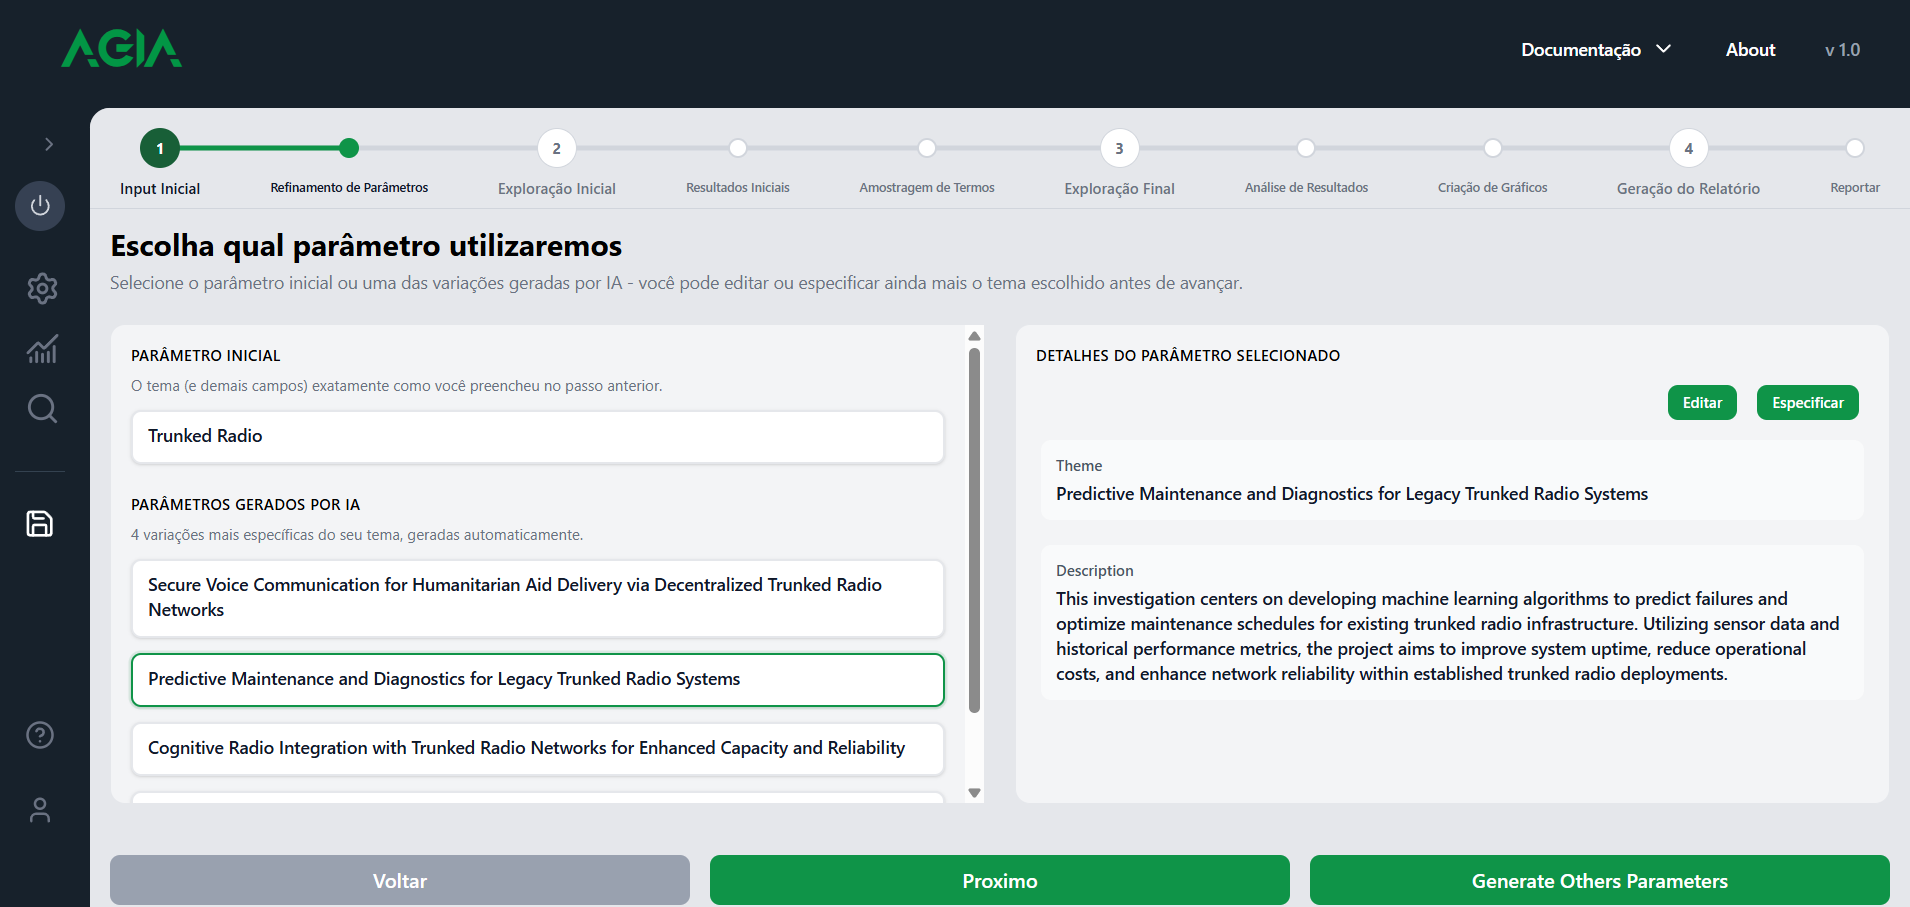
\includegraphics[keepaspectratio,alt={Tela de refinamento com o parâmetro inicial, as variações geradas pela IA e os detalhes da variação selecionada.}]{imagens/03-refinamento.png}}
\caption{Tela de refinamento com o parâmetro inicial, as variações
geradas pela IA e os detalhes da variação selecionada.}
\end{figure}

\begin{itemize}
\tightlist
\item
  À esquerda, \textbf{Parâmetro inicial} mostra o tema como você
  preencheu. Abaixo, \textbf{Parâmetros gerados por IA} lista quatro
  variações mais específicas.
\item
  À direita, \textbf{Detalhes do parâmetro selecionado} mostra o tema e
  a descrição da variação escolhida, com os botões \textbf{Editar} e
  \textbf{Especificar}.

  \begin{itemize}
  \tightlist
  \item
    \textbf{Editar} permite alterar o texto manualmente, sem custo de
    IA.
  \item
    \textbf{Especificar} pede à IA que refine ainda mais a variação
    selecionada.
  \end{itemize}
\item
  No rodapé: \textbf{Voltar}, \textbf{Próximo} e \textbf{Generate Others
  Parameters}. Este último rótulo está em inglês na versão de
  desenvolvimento e gera um novo conjunto de variações.
\end{itemize}

Quanto mais específica a variação, mais afunilada a busca, e ela pode
retornar poucos resultados. Se isso acontecer, volte e escolha uma
variação mais ampla.

Reabrir a tela sem ter mudado o formulário reaproveita as variações já
geradas. Para gerar variações novas, altere o formulário e clique em
\textbf{Refinar parâmetros} de novo.

\begin{center}\rule{0.5\linewidth}{0.5pt}\end{center}

\chapter{5. Etapa 2 --- Exploração
inicial}\label{etapa-2-explorauxe7uxe3o-inicial}

O objetivo desta etapa é \textbf{descobrir o campo}: uma busca restrita,
com amostra pequena, para encontrar um primeiro conjunto de documentos
de referência. A partir deles, o sistema extrai os termos que vão compor
a busca final.

\section{5.1 Escolha da query}\label{escolha-da-query}

A tela mostra duas seções independentes, uma para \textbf{patentes
(OPS)} e outra para \textbf{artigos (Scopus)}. Cada uma traz
\textbf{queries iniciais geradas por IA}, em opções numeradas (Opção 1,
Opção 2 etc.).

\begin{figure}
\centering
\pandocbounded{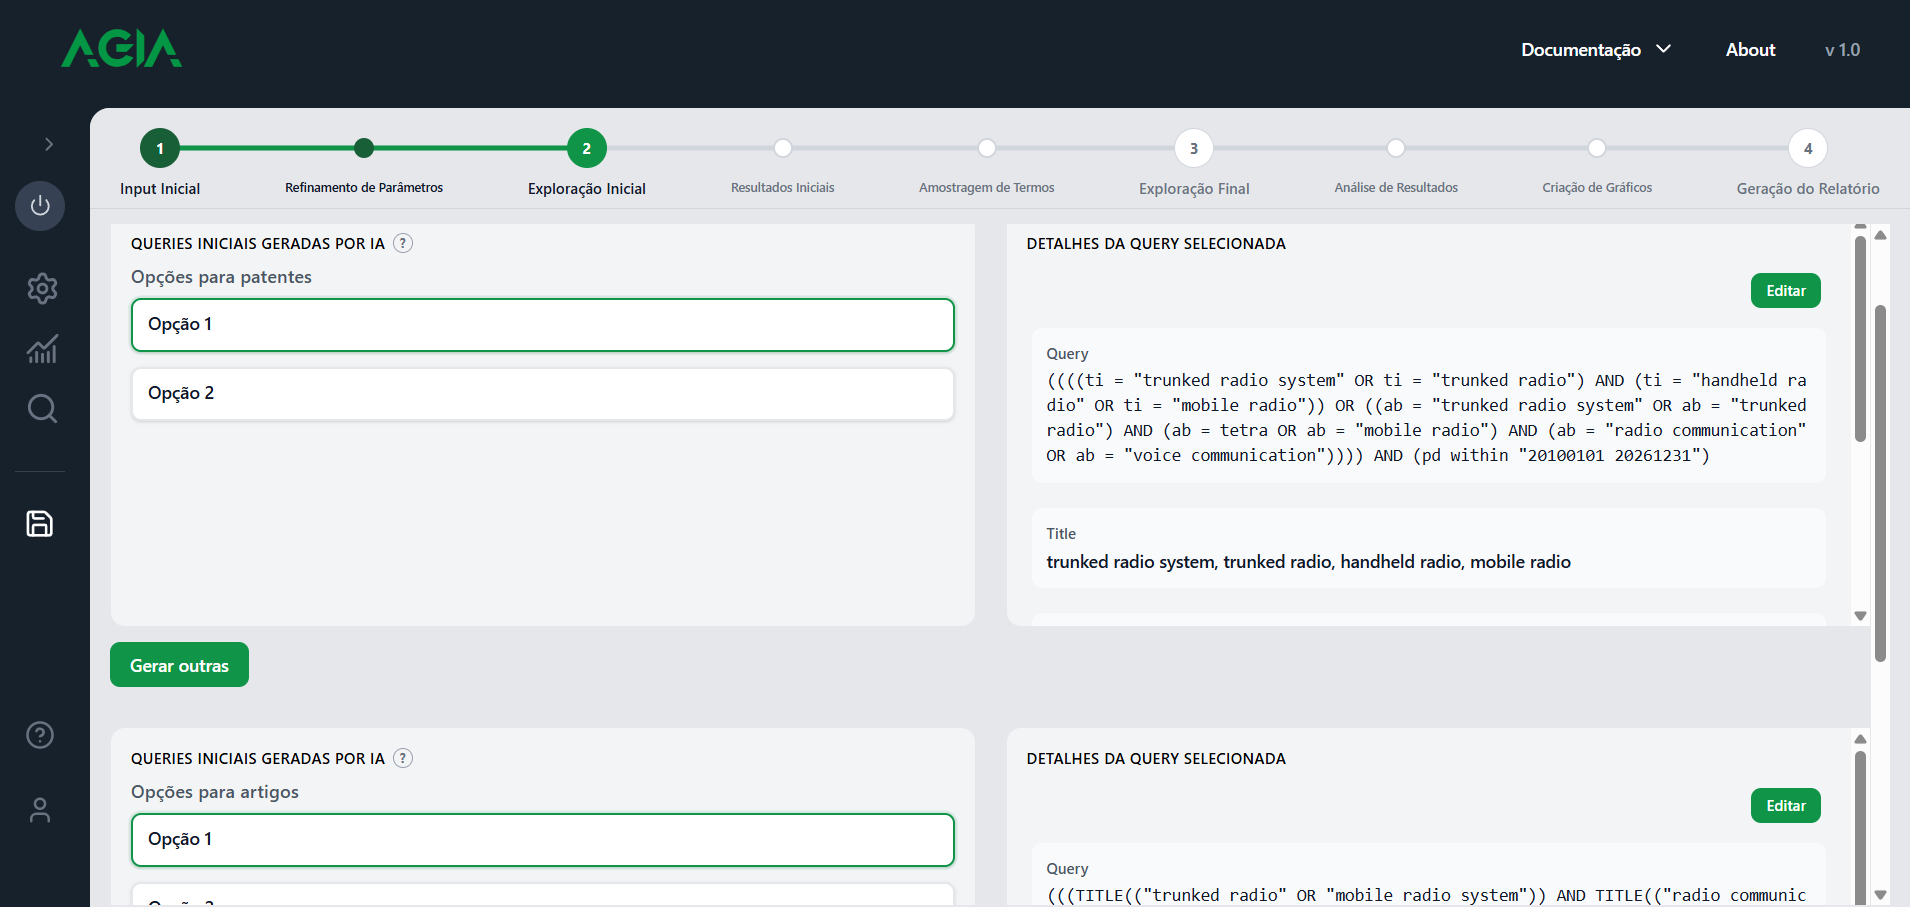
\includegraphics[keepaspectratio,alt={Queries iniciais geradas por IA para patentes e artigos, com os detalhes da query selecionada.}]{imagens/04-queries-iniciais.png}}
\caption{Queries iniciais geradas por IA para patentes e artigos, com os
detalhes da query selecionada.}
\end{figure}

\begin{itemize}
\tightlist
\item
  Clique numa opção para ver sua \textbf{query} completa (a expressão
  booleana) e o \textbf{título} com os termos usados.
\item
  \textbf{Editar} abre a query para alteração manual.
\item
  \textbf{Gerar outras} pede novas opções à IA para aquela base.
\item
  O \textbf{medidor de complexidade} avisa quando uma query tende a
  falhar ou a não trazer resultados. Queries muito longas ou muito
  aninhadas costumam zerar a busca. Simplifique a query se o medidor
  indicar complexidade alta.
\end{itemize}

\textbf{Próximo} executa a busca exploratória com as queries escolhidas.
Se a mesma query já foi buscada antes, o sistema reaproveita os
resultados.

\section{5.2 Resultados iniciais}\label{resultados-iniciais}

Tela somente leitura, com a amostra de patentes (à esquerda) e de
artigos (à direita) trazida pela busca exploratória.

\begin{figure}
\centering
\pandocbounded{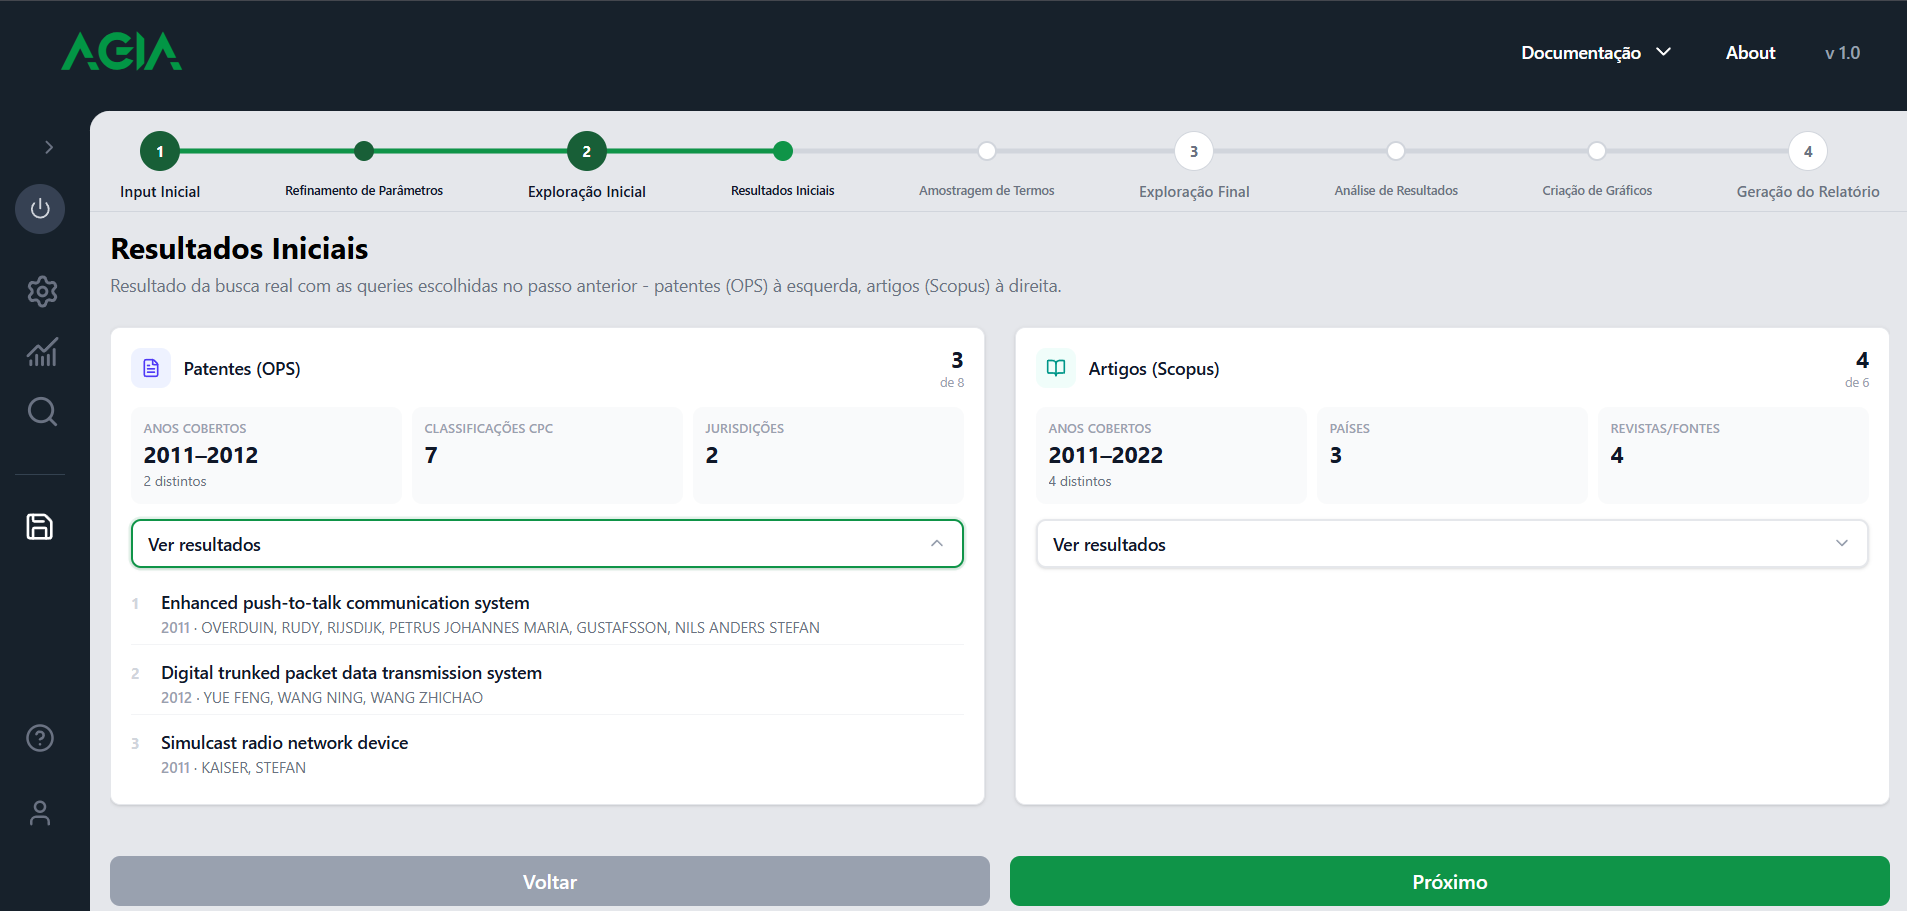
\includegraphics[keepaspectratio,alt={Resultados iniciais: patentes (OPS) à esquerda e artigos (Scopus) à direita.}]{imagens/05-resultados-iniciais.png}}
\caption{Resultados iniciais: patentes (OPS) à esquerda e artigos
(Scopus) à direita.}
\end{figure}

Cada cartão mostra o número de documentos encontrados e alguns
indicadores: para patentes, os anos cobertos, as classificações CPC e as
jurisdições; para artigos, os anos cobertos, os países e as revistas ou
fontes. \textbf{Ver resultados} expande a lista de documentos, com
título, ano e autores.

Use esta tela para conferir se o campo está certo. Se os documentos não
têm relação com o tema, volte e ajuste o refinamento ou a query.

\section{5.3 Amostragem de termos}\label{amostragem-de-termos}

Os termos são \textbf{extraídos automaticamente} dos títulos e resumos
da amostra, por processamento de linguagem local. \textbf{Não há IA
generativa nesta etapa}: os mesmos documentos sempre produzem os mesmos
termos. Por isso não existe ``gerar outros termos''. Para obter outros,
mude a query exploratória.

\begin{figure}
\centering
\pandocbounded{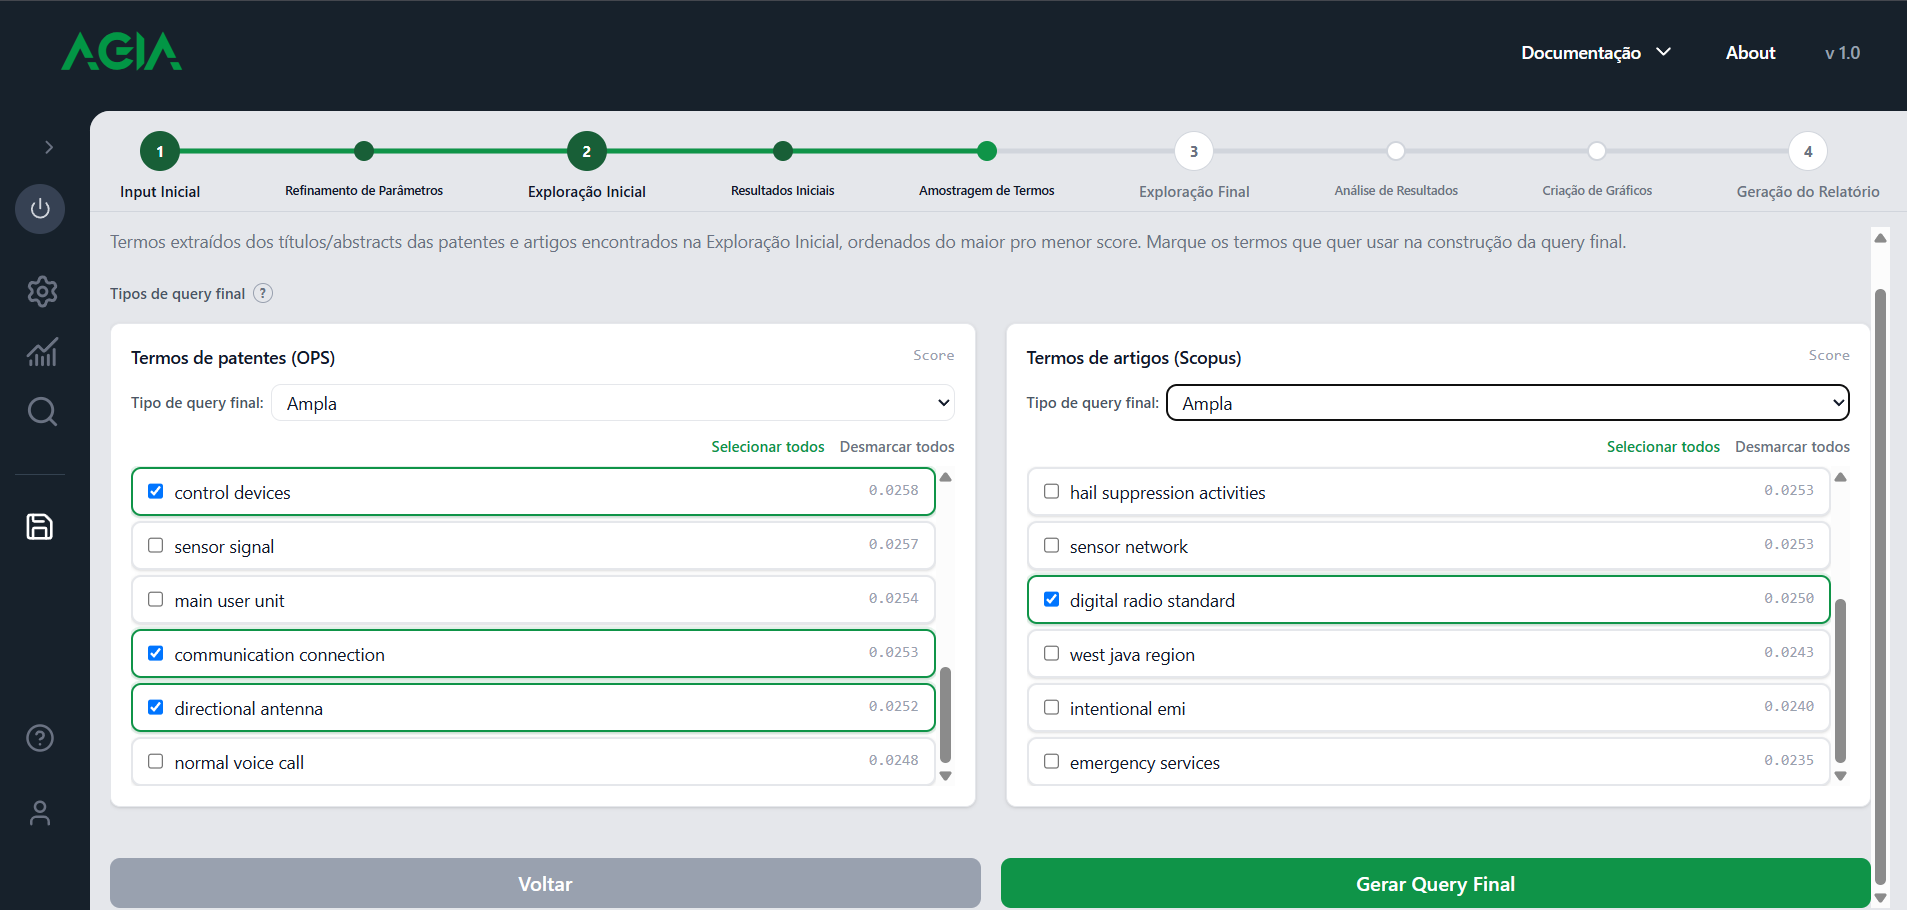
\includegraphics[keepaspectratio,alt={Amostragem de termos para patentes e artigos, com o tipo de query final e os scores de cada termo.}]{imagens/06-termos.png}}
\caption{Amostragem de termos para patentes e artigos, com o tipo de
query final e os scores de cada termo.}
\end{figure}

Os termos aparecem \textbf{ordenados por score}, do maior para o menor,
em duas colunas (patentes e artigos). Para cada termo:

\begin{itemize}
\tightlist
\item
  \textbf{Marque} os que devem entrar na query final. \textbf{Selecionar
  todos} e \textbf{Desmarcar todos} agilizam a escolha.
\item
  O \textbf{Tipo de query final} (Específica, Balanceada ou Ampla)
  define a abrangência da busca final:

  \begin{itemize}
  \tightlist
  \item
    \textbf{Específica} --- busca mais restrita, com menos ruído e menos
    resultados;
  \item
    \textbf{Balanceada} --- meio-termo;
  \item
    \textbf{Ampla} --- busca mais abrangente, com mais resultados e mais
    ruído.
  \end{itemize}
\end{itemize}

Clique em \textbf{Gerar Query Final} para a IA montar a query da próxima
etapa. A IA só é chamada de novo se os termos marcados ou o tipo mudaram
desde a última geração.

\begin{center}\rule{0.5\linewidth}{0.5pt}\end{center}

\chapter{6. Etapa 3 --- Exploração
final}\label{etapa-3-explorauxe7uxe3o-final}

\section{6.1 Revisão da query final}\label{revisuxe3o-da-query-final}

A tela mostra a query final gerada para cada base, montada a partir do
tipo e dos termos escolhidos.

\begin{figure}
\centering
\pandocbounded{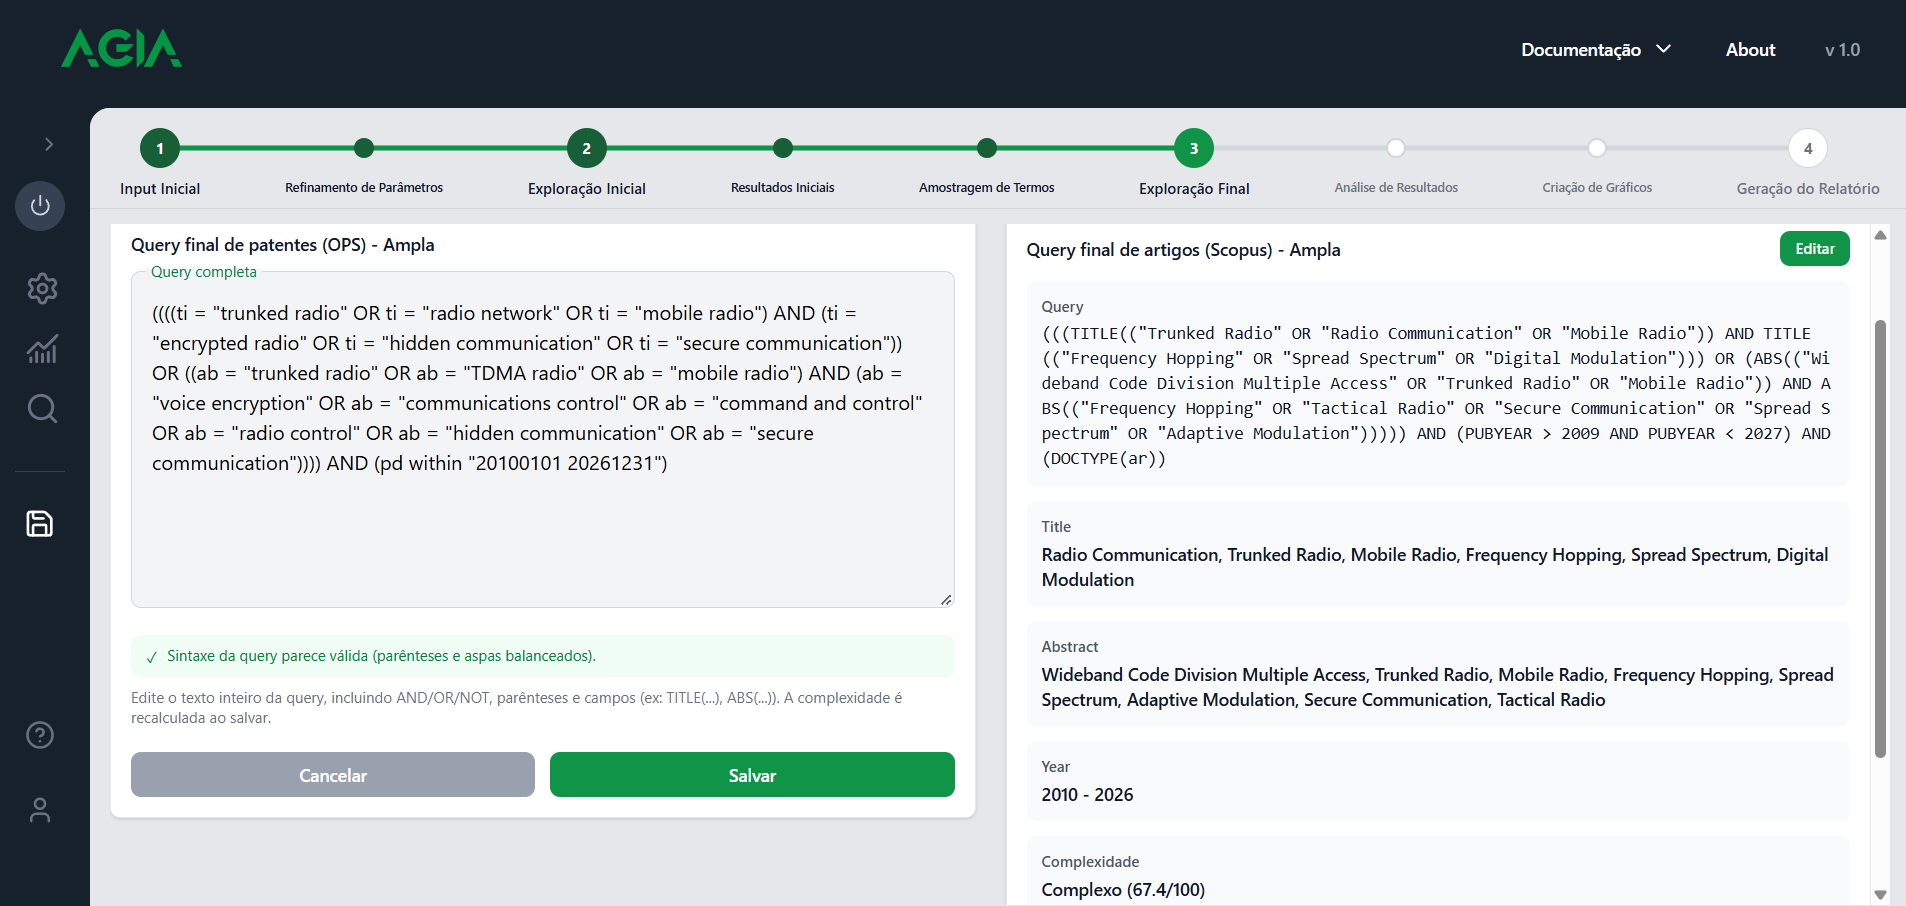
\includegraphics[keepaspectratio,alt={Query final de patentes e de artigos, com a validação de sintaxe e os indicadores de complexidade.}]{imagens/07-query-final.png}}
\caption{Query final de patentes e de artigos, com a validação de
sintaxe e os indicadores de complexidade.}
\end{figure}

\begin{itemize}
\tightlist
\item
  A query de patentes aparece num campo editável, com a indicação
  \textbf{Sintaxe da query parece válida} quando parênteses e aspas
  estão balanceados. Edite a query, se quiser, e use \textbf{Salvar}. A
  complexidade é recalculada ao salvar.
\item
  A query de artigos aparece à direita, com os campos \textbf{Title},
  \textbf{Abstract}, \textbf{Year} e \textbf{Complexidade}. Por exemplo,
  ``Complexo (67,4/100)'' indica uma query com nota alta de
  complexidade.
\item
  \textbf{Gerar de novo} cria outra versão da query.
\item
  \textbf{Confirmar e buscar} executa a \textbf{busca final}. Ela sempre
  roda, mesmo que a mesma query já tenha sido buscada.
\end{itemize}

Use \textbf{Confirmar e buscar} com cuidado: é a busca que alimenta
todas as análises e o relatório.

Se a busca não trouxer nenhum resultado, a tela informa isso. Volte à
revisão, amplie a query (variante \textbf{Ampla} ou mais termos) e tente
de novo.

\section{6.2 Análise de resultados}\label{anuxe1lise-de-resultados}

Estatísticas agregadas da busca final, uma seção para cada base.

\begin{figure}
\centering
\pandocbounded{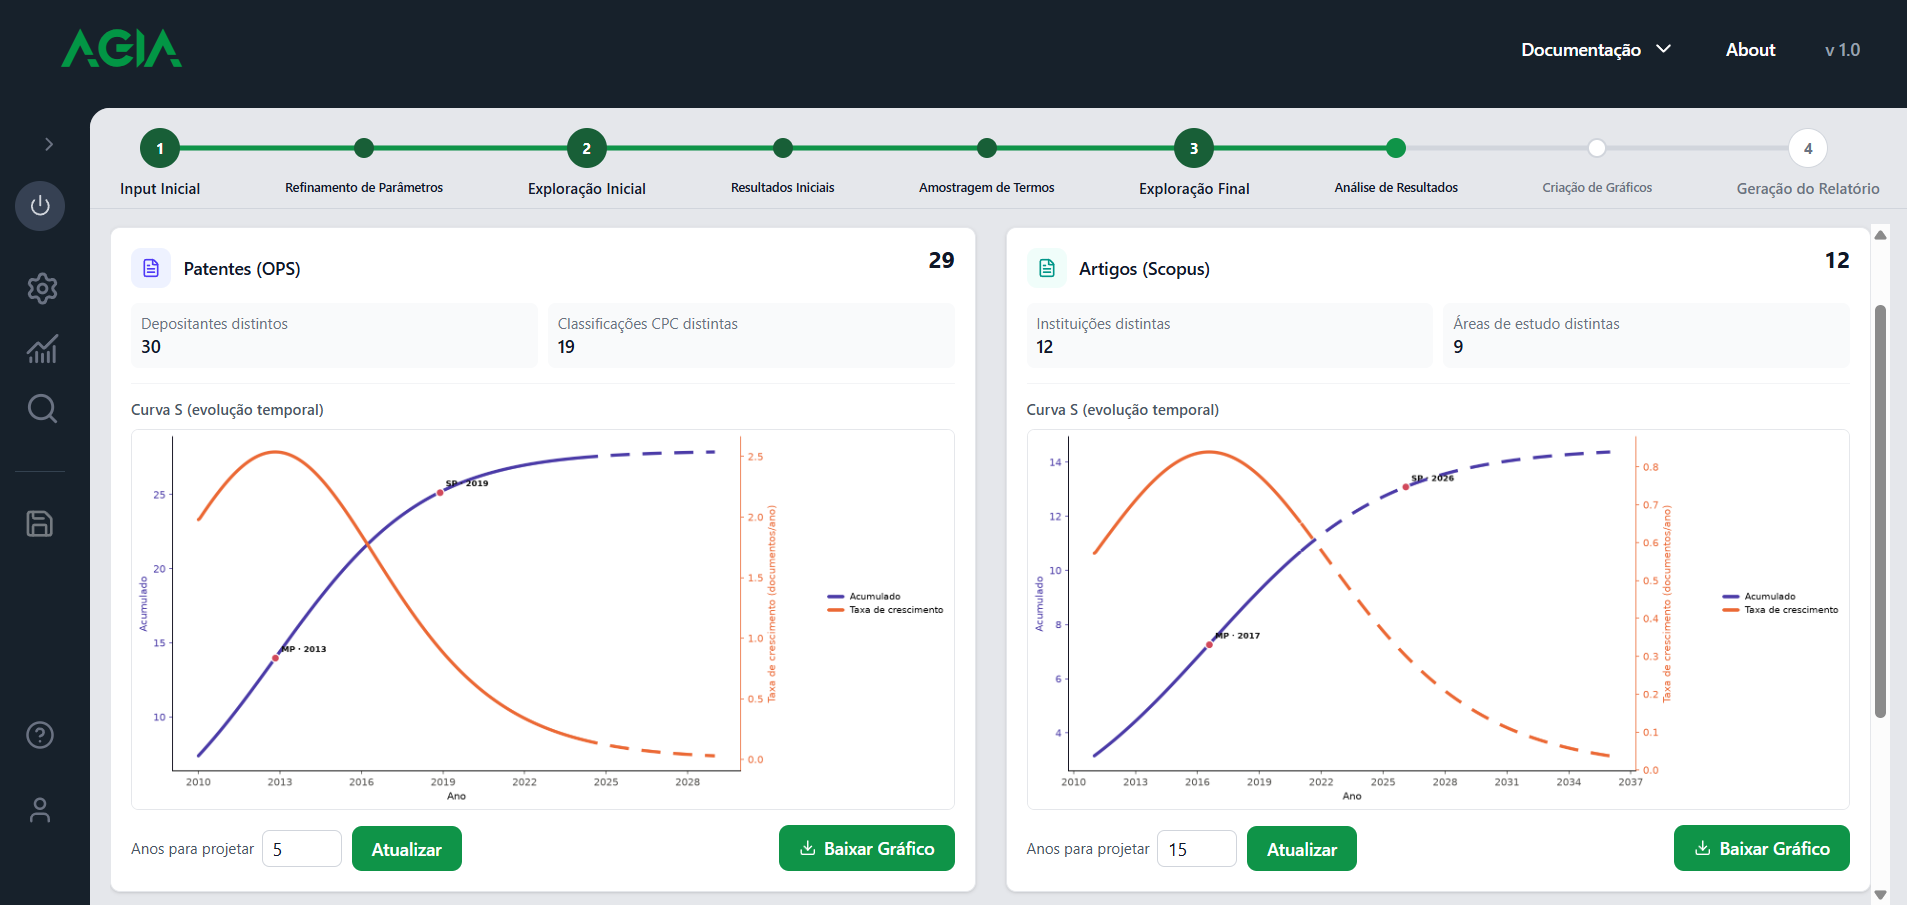
\includegraphics[keepaspectratio,alt={Análise de resultados com os indicadores de patentes e artigos e as curvas S de cada base.}]{imagens/08-analise-curvas.png}}
\caption{Análise de resultados com os indicadores de patentes e artigos
e as curvas S de cada base.}
\end{figure}

\begin{itemize}
\tightlist
\item
  \textbf{Patentes (OPS):} depositantes distintos e classificações CPC
  distintas.
\item
  \textbf{Artigos (Scopus):} instituições distintas e áreas de estudo
  distintas.
\item
  Cada cartão também exibe um número grande no canto superior direito. A
  captura não deixa explícito o que ele representa; confira o
  significado na versão em uso.
\end{itemize}

\textbf{Curva S (evolução temporal)}, mostrada para cada base:

\begin{itemize}
\tightlist
\item
  A linha \textbf{Acumulado} mostra o total de documentos ao longo dos
  anos. A linha \textbf{Taxa de crescimento} mostra quão rápido o volume
  cresce.
\item
  Os pontos marcados (\textbf{MP} e \textbf{SP}, e \textbf{GP} quando
  aparece) indicam fases do ciclo de vida da tecnologia.
\item
  \textbf{Anos para projetar} define quantos anos à frente a curva é
  estendida. A parte tracejada é a projeção. Clique em
  \textbf{Atualizar} para recalcular.
\item
  \textbf{Baixar Gráfico} salva a imagem da curva.
\end{itemize}

Quando o ajuste não é confiável, o gráfico mostra um \textbf{aviso}
explicando o motivo. Nesse caso, a curva continua visível, sem a parte
projetada, e deve ser lida com cautela. Buscas com mais anos e mais
documentos costumam resolver.

\section{6.3 Criação de gráficos}\label{criauxe7uxe3o-de-gruxe1ficos}

Esta tela é \textbf{automática}:

\begin{enumerate}
\def\labelenumi{\arabic{enumi}.}
\tightlist
\item
  salva a sessão;
\item
  roda a \textbf{inferência estatística}, que verifica se a amostra
  cobre bem a diversidade do campo e se os rankings são estáveis;
\item
  se a amostra for insuficiente, pede mais resultados à busca final, até
  saturar ou até o tempo máximo configurado;
\item
  gera os gráficos: top depositantes e instituições, distribuição de CPC
  e de áreas de estudo, histórico anual e curva S.
\end{enumerate}

Ao terminar, a tela avança sozinha para a Geração do Relatório.

\begin{itemize}
\tightlist
\item
  Se algo falhar, a tela mostra o erro com a opção \textbf{Tentar
  novamente}.
\item
  Gráficos já gerados são reaproveitados: voltar a esta tela sem mudar a
  busca final \textbf{não refaz o trabalho}.
\end{itemize}

\begin{center}\rule{0.5\linewidth}{0.5pt}\end{center}

\chapter{7. Etapa 4 --- Geração do
relatório}\label{etapa-4-gerauxe7uxe3o-do-relatuxf3rio}

Esta etapa tem três partes: os metadados, as seções de texto e a
montagem do documento.

\section{7.1 Metadados do REPTEC}\label{metadados-do-reptec}

Preencha os dados que aparecem na capa e nas assinaturas.

\begin{figure}
\centering
\pandocbounded{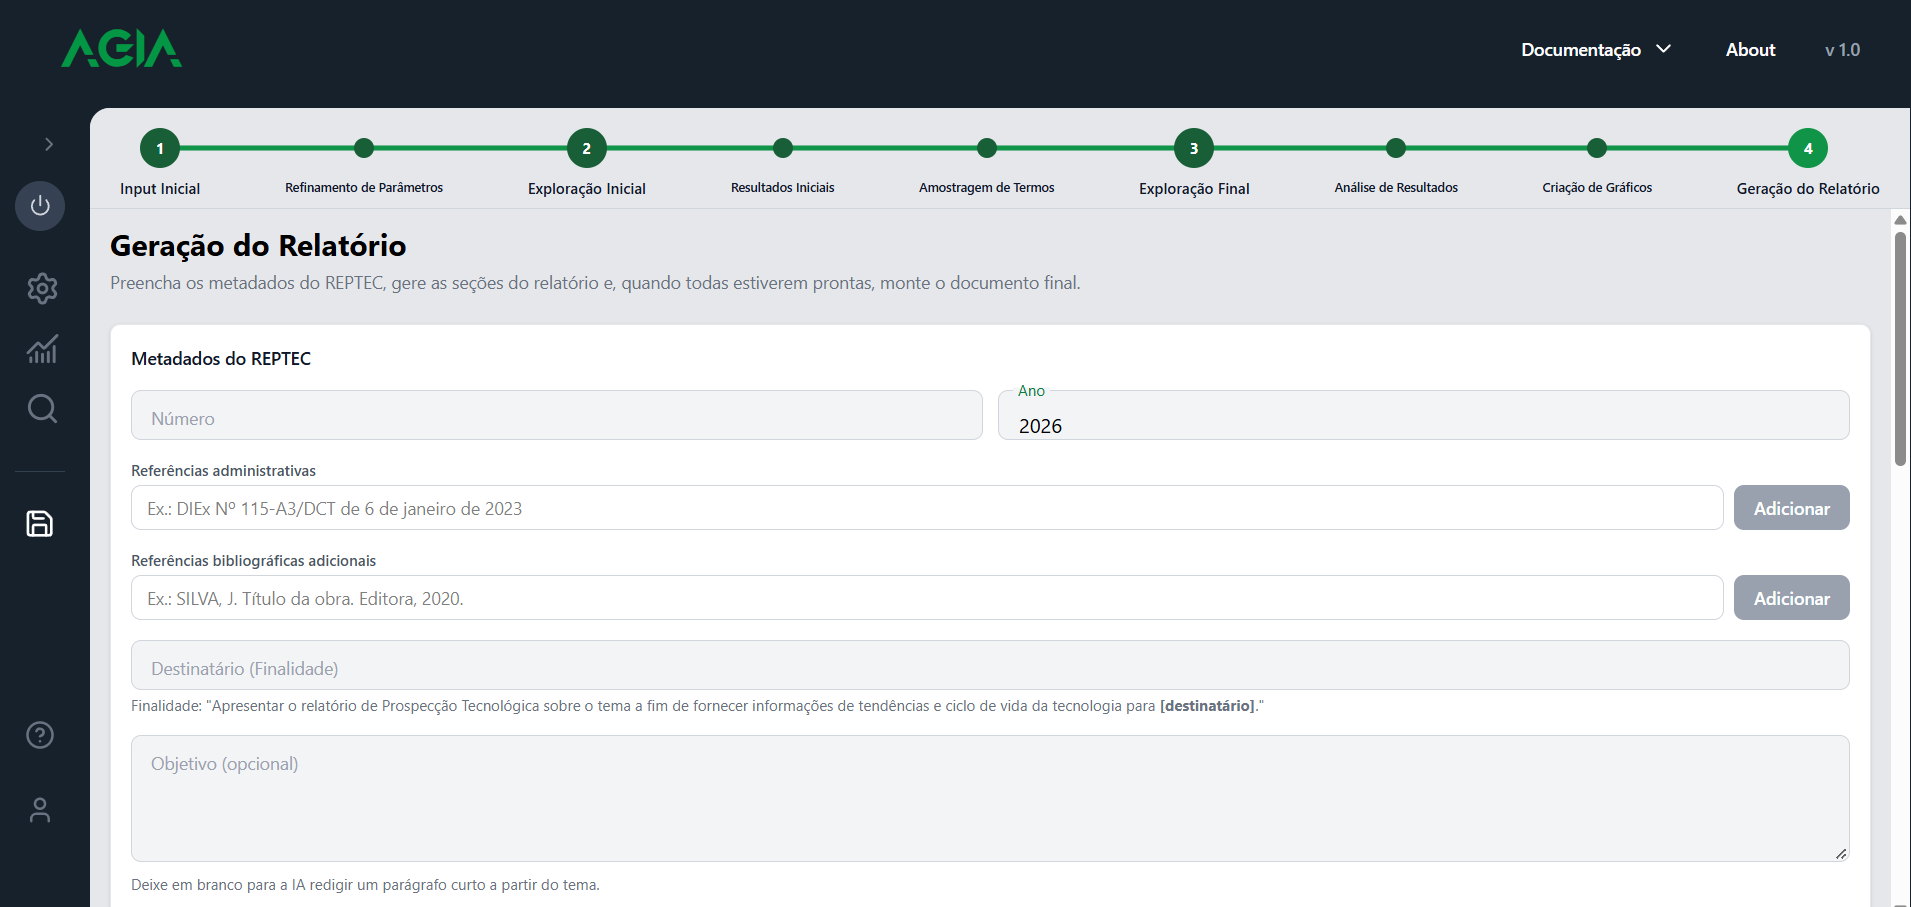
\includegraphics[keepaspectratio,alt={Formulário de metadados do REPTEC: número, ano, referências, destinatário e objetivo.}]{imagens/09-metadados.png}}
\caption{Formulário de metadados do REPTEC: número, ano, referências,
destinatário e objetivo.}
\end{figure}

{\def\LTcaptype{none} % do not increment counter
\begin{longtable}[]{@{}
  >{\raggedright\arraybackslash}p{(\linewidth - 2\tabcolsep) * \real{0.4000}}
  >{\raggedright\arraybackslash}p{(\linewidth - 2\tabcolsep) * \real{0.6000}}@{}}
\toprule\noalign{}
\begin{minipage}[b]{\linewidth}\raggedright
Campo
\end{minipage} & \begin{minipage}[b]{\linewidth}\raggedright
Observação
\end{minipage} \\
\midrule\noalign{}
\endhead
\bottomrule\noalign{}
\endlastfoot
\textbf{Número} & Ex.: ``001''. \\
\textbf{Ano} & Vem preenchido com o ano atual (2026 na captura). \\
\textbf{Referências administrativas} & Ex.: ``DIEx Nº 115-A3/DCT de 6 de
janeiro de 2023''. Use \textbf{Adicionar} para incluir cada
referência. \\
\textbf{Referências bibliográficas adicionais} & Em ABNT. Ex.: ``SILVA,
J. Título da obra. Editora, 2020.'' Use \textbf{Adicionar} para cada
item. \\
\textbf{Destinatário (Finalidade)} & Para quem é o relatório.
Obrigatório. A frase de finalidade mostra o campo
\texttt{{[}destinatário{]}}, preenchido a partir deste campo. \\
\textbf{Objetivo} & Opcional. Se ficar vazio, a IA escreve um parágrafo
curto a partir do tema. \\
\textbf{Local} & Linha antes das assinaturas. Ex.: ``Rio de
Janeiro''. \\
\textbf{Assinaturas} & Elaborado, Revisado e Aprovado por:
\textbf{nome}, \textbf{posto/graduação} e \textbf{função}. \\
\end{longtable}
}

Regras de validação:

\begin{itemize}
\tightlist
\item
  Valores de preenchimento como ``teste'' ou ``sdasd'' são
  \textbf{recusados}.
\item
  \textbf{Elaborado por é obrigatório.} Revisado e Aprovado por podem
  ficar vazios.
\item
  Pelo menos um assinante, com nome, posto/graduação e função, é
  obrigatório.
\item
  Use \textbf{Remover} para apagar uma linha de assinatura.
\end{itemize}

Confira os dados antes de montar o documento: o texto gerado pela IA
pode não bater com os dados se algo for alterado depois.

\section{7.2 Seções do relatório}\label{seuxe7uxf5es-do-relatuxf3rio}

\textbf{Continuar geração} (no canto superior direito) gera, em
sequência, as seções que ainda estão pendentes. Cada seção também tem
seu botão de play, para gerar uma seção específica.

\begin{figure}
\centering
\pandocbounded{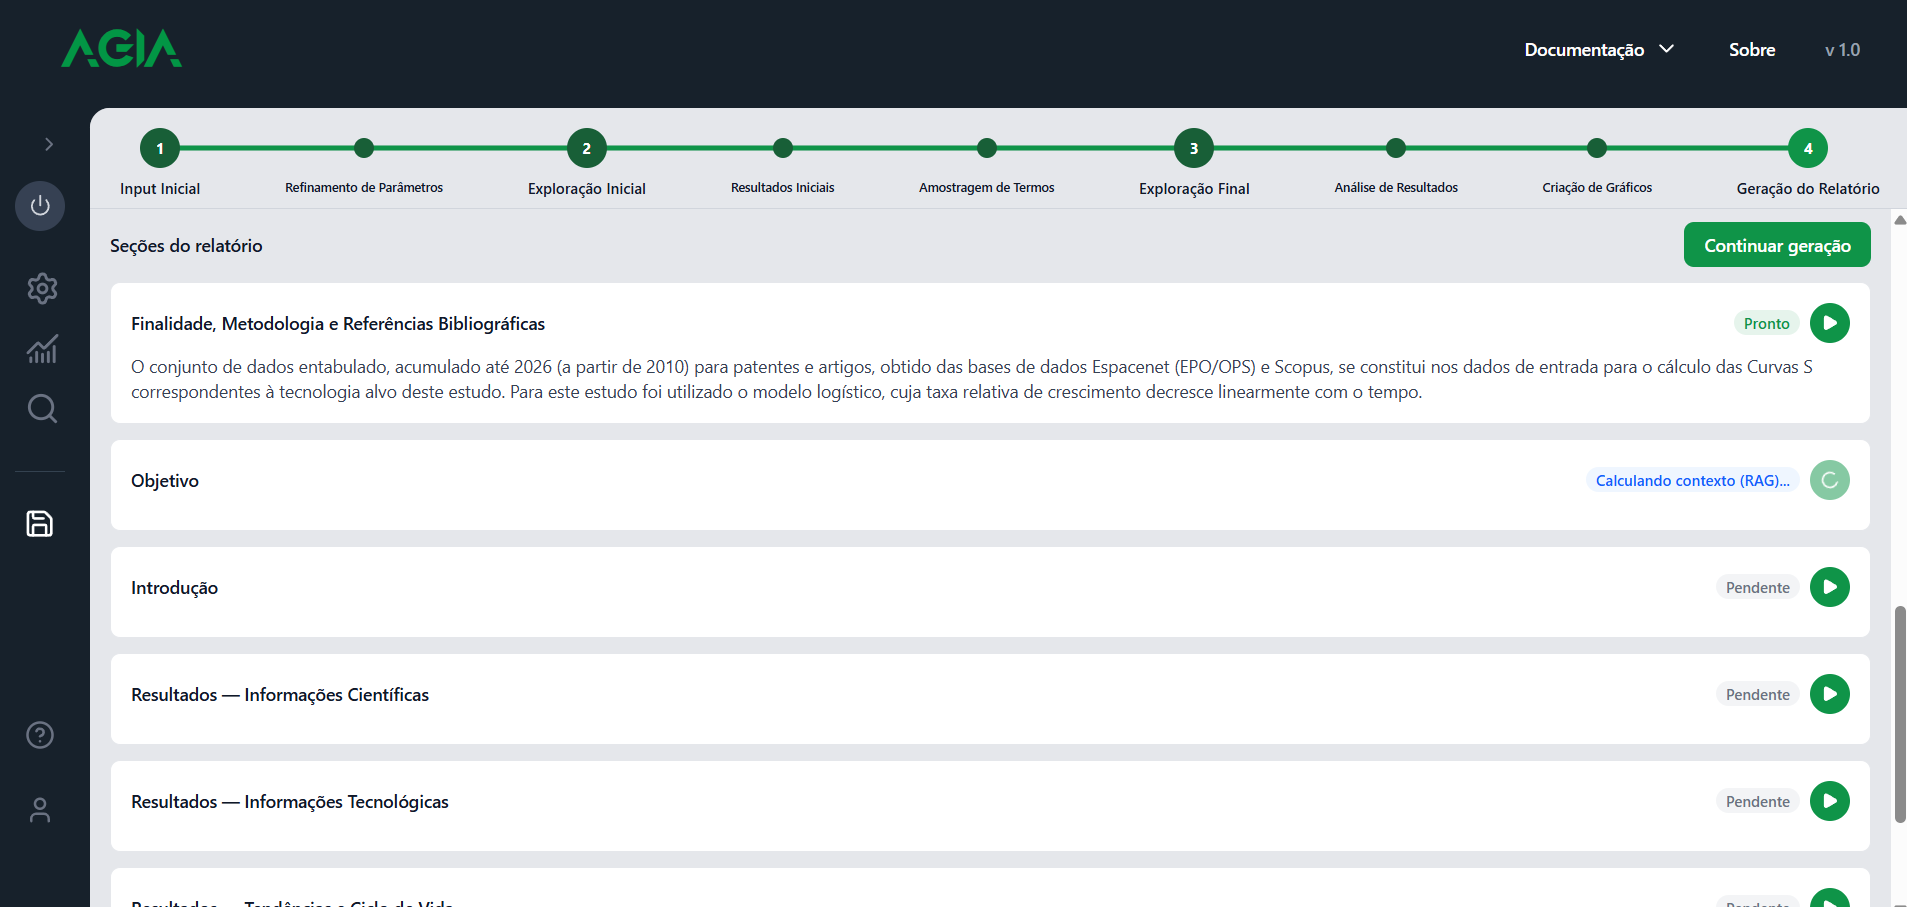
\includegraphics[keepaspectratio,alt={Lista de seções do relatório com o status de cada uma: pronta, calculando contexto ou pendente.}]{imagens/10-secoes.png}}
\caption{Lista de seções do relatório com o status de cada uma: pronta,
calculando contexto ou pendente.}
\end{figure}

As seções são:

\begin{itemize}
\tightlist
\item
  \textbf{Finalidade, Metodologia e Referências Bibliográficas} ---
  montada pelo sistema a partir dos dados do estudo; o texto de
  metodologia não é gerado pela IA.
\item
  \textbf{Objetivo}, \textbf{Introdução}, \textbf{Resultados ---
  Informações Científicas}, \textbf{Resultados --- Informações
  Tecnológicas} e \textbf{Resultados --- Tendências e Ciclo de Vida} ---
  textos gerados pela IA, com base nos trechos mais relevantes dos
  documentos e gráficos da busca.
\end{itemize}

Cada seção mostra seu andamento: \textbf{Calculando contexto (RAG)}
(busca, nos resultados, os trechos mais relevantes para a seção), depois
\textbf{gerando texto}, até ficar \textbf{Pronto}. Se uma seção falhar,
use \textbf{Continuar geração} ou gere-a de novo.

Para cada seção, o texto cita os documentos recuperados. O sistema
remove citações que não correspondam a um documento desse contexto,
então um documento pouco relevante para a seção pode não aparecer.

\section{7.3 Montar o .tex}\label{montar-o-.tex}

\textbf{Montar .tex} monta o documento LaTeX com as seções e os gráficos
e \textbf{abre o editor}.

\begin{quote}
\textbf{Atenção:} montar o .tex \textbf{conclui a sessão}. A partir daí,
a pesquisa (queries, termos e buscas) não pode mais ser editada, só o
texto do relatório.
\end{quote}

Para refazer o documento do zero, use \textbf{Remontar .tex} no editor.
Ele pede confirmação e \textbf{descarta as edições manuais}.

\begin{center}\rule{0.5\linewidth}{0.5pt}\end{center}

\chapter{8. Editor do relatório}\label{editor-do-relatuxf3rio}

O editor é onde o relatório ganha a forma final.

\begin{figure}
\centering
\pandocbounded{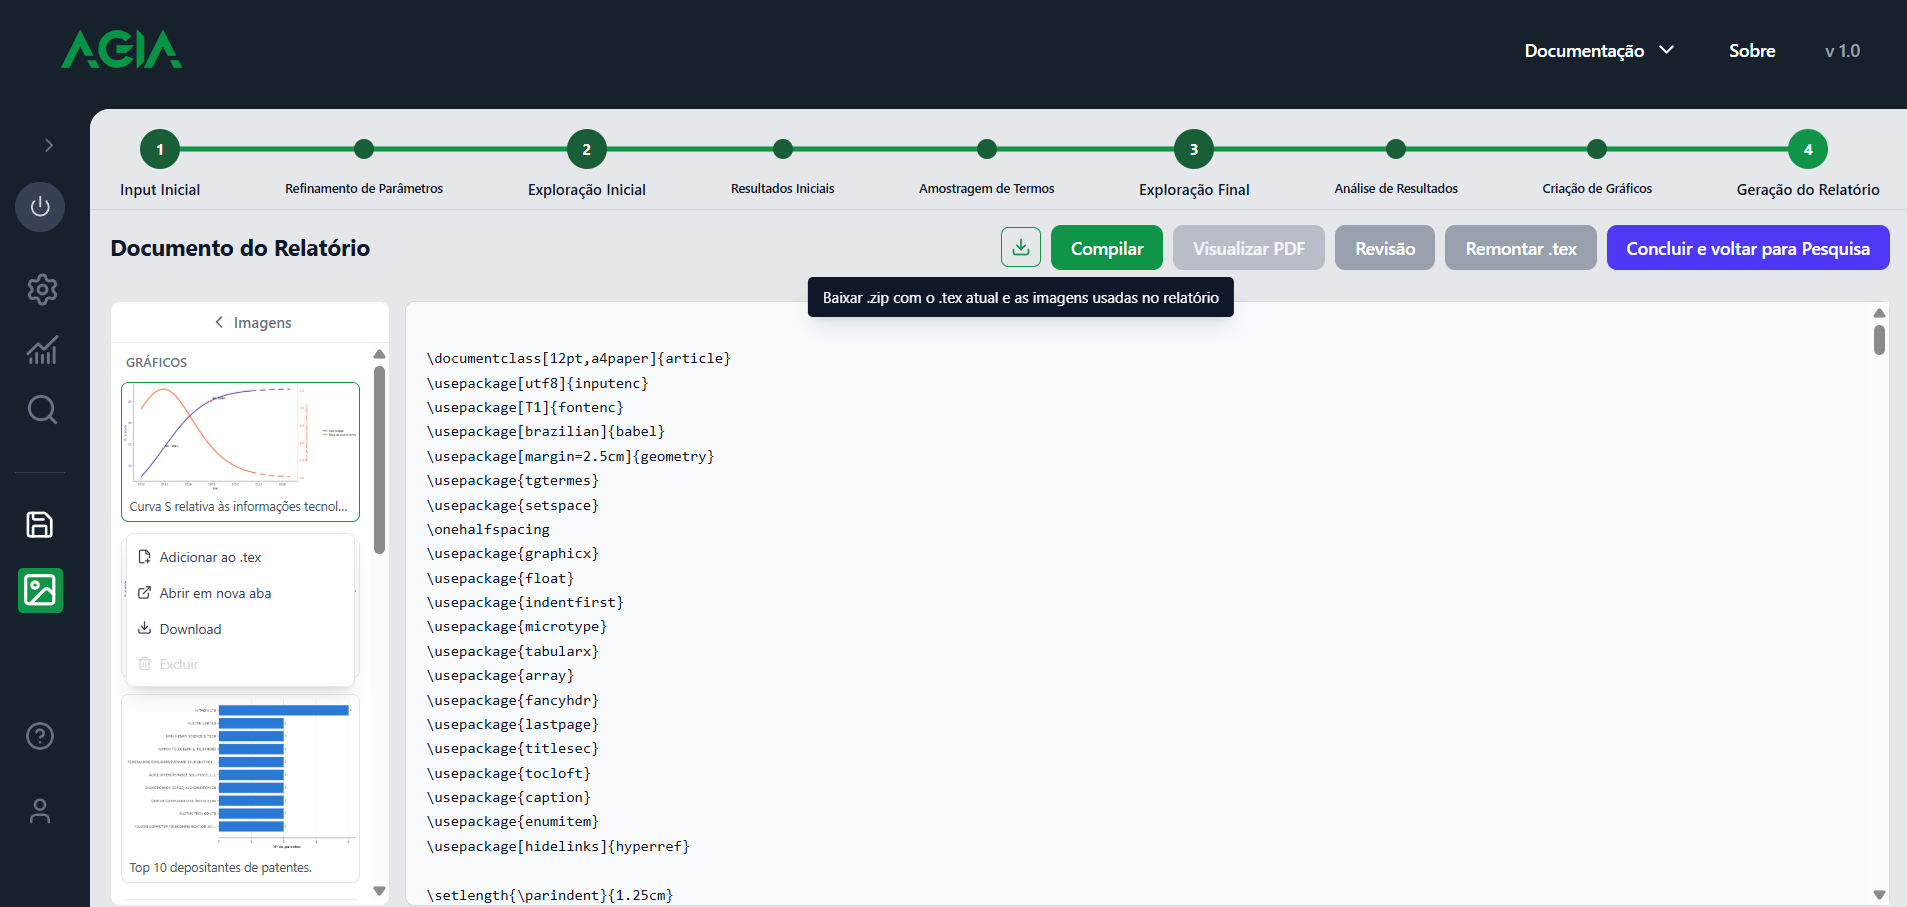
\includegraphics[keepaspectratio,alt={Editor do relatório: barra de ações, painel de imagens à esquerda e o código LaTeX ao centro.}]{imagens/11-editor.png}}
\caption{Editor do relatório: barra de ações, painel de imagens à
esquerda e o código LaTeX ao centro.}
\end{figure}

\section{8.1 Barra de ações}\label{barra-de-auxe7uxf5es}

\begin{itemize}
\tightlist
\item
  \textbf{Baixar} (ícone de download) --- baixa um
  \texttt{.}\allowbreak{}\texttt{zip} com o
  \texttt{.}\allowbreak{}\texttt{tex} atual e as imagens usadas no
  relatório, para compilar ou editar fora do sistema.
\item
  \textbf{Compilar} --- gera o PDF a partir do
  \texttt{.}\allowbreak{}\texttt{tex}.
\item
  \textbf{Visualizar PDF} --- abre a última versão compilada. Fica
  desabilitado até a primeira compilação.
\item
  \textbf{Revisão} --- abre o painel de revisão (seção 8.3).
\item
  \textbf{Remontar .tex} --- refaz o documento do zero e descarta as
  edições manuais.
\item
  \textbf{Concluir e voltar para Pesquisa} --- encerra o fluxo e abre a
  tela de Busca.
\end{itemize}

\textbf{Compilar, revisar, inserir imagens e baixar o .zip nunca
descartam as suas edições.} Só \textbf{Remontar .tex} faz isso.

\section{8.2 Painel de imagens}\label{painel-de-imagens}

O painel \textbf{Imagens}, à esquerda, lista as figuras disponíveis, em
\textbf{Gráficos} (os gerados pela busca) e em \textbf{Anexos} (imagens
que você envia).

Para cada imagem, o menu oferece:

\begin{itemize}
\tightlist
\item
  \textbf{Adicionar ao .tex} --- insere a figura na posição do cursor,
  no formato do relatório.
\item
  \textbf{Abrir em nova aba} --- mostra a imagem em tamanho real.
\item
  \textbf{Download} --- baixa a imagem.
\item
  \textbf{Excluir} --- remove um anexo. Gráficos gerados pelo sistema
  não podem ser excluídos.
\end{itemize}

Para incluir uma imagem própria, use o botão \textbf{+} ao lado de
\textbf{Anexos}. Para anexos, o título entra como ``Título da figura'',
para você substituir.

\begin{quote}
Excluir um anexo que ainda é referenciado no
\texttt{.}\allowbreak{}\texttt{tex} faz a compilação falhar com
``arquivo não encontrado''. Remova a referência antes de excluir.
\end{quote}

\section{8.3 Revisão}\label{revisuxe3o}

O botão \textbf{Revisão} abre o painel \textbf{Revisão}, à direita. Ele
mostra sugestões de correção de ortografia, acentuação, concordância e
LaTeX, indicando a origem de cada uma (por exemplo, LanguageTool) e a
seção em que aparece.

\begin{figure}
\centering
\pandocbounded{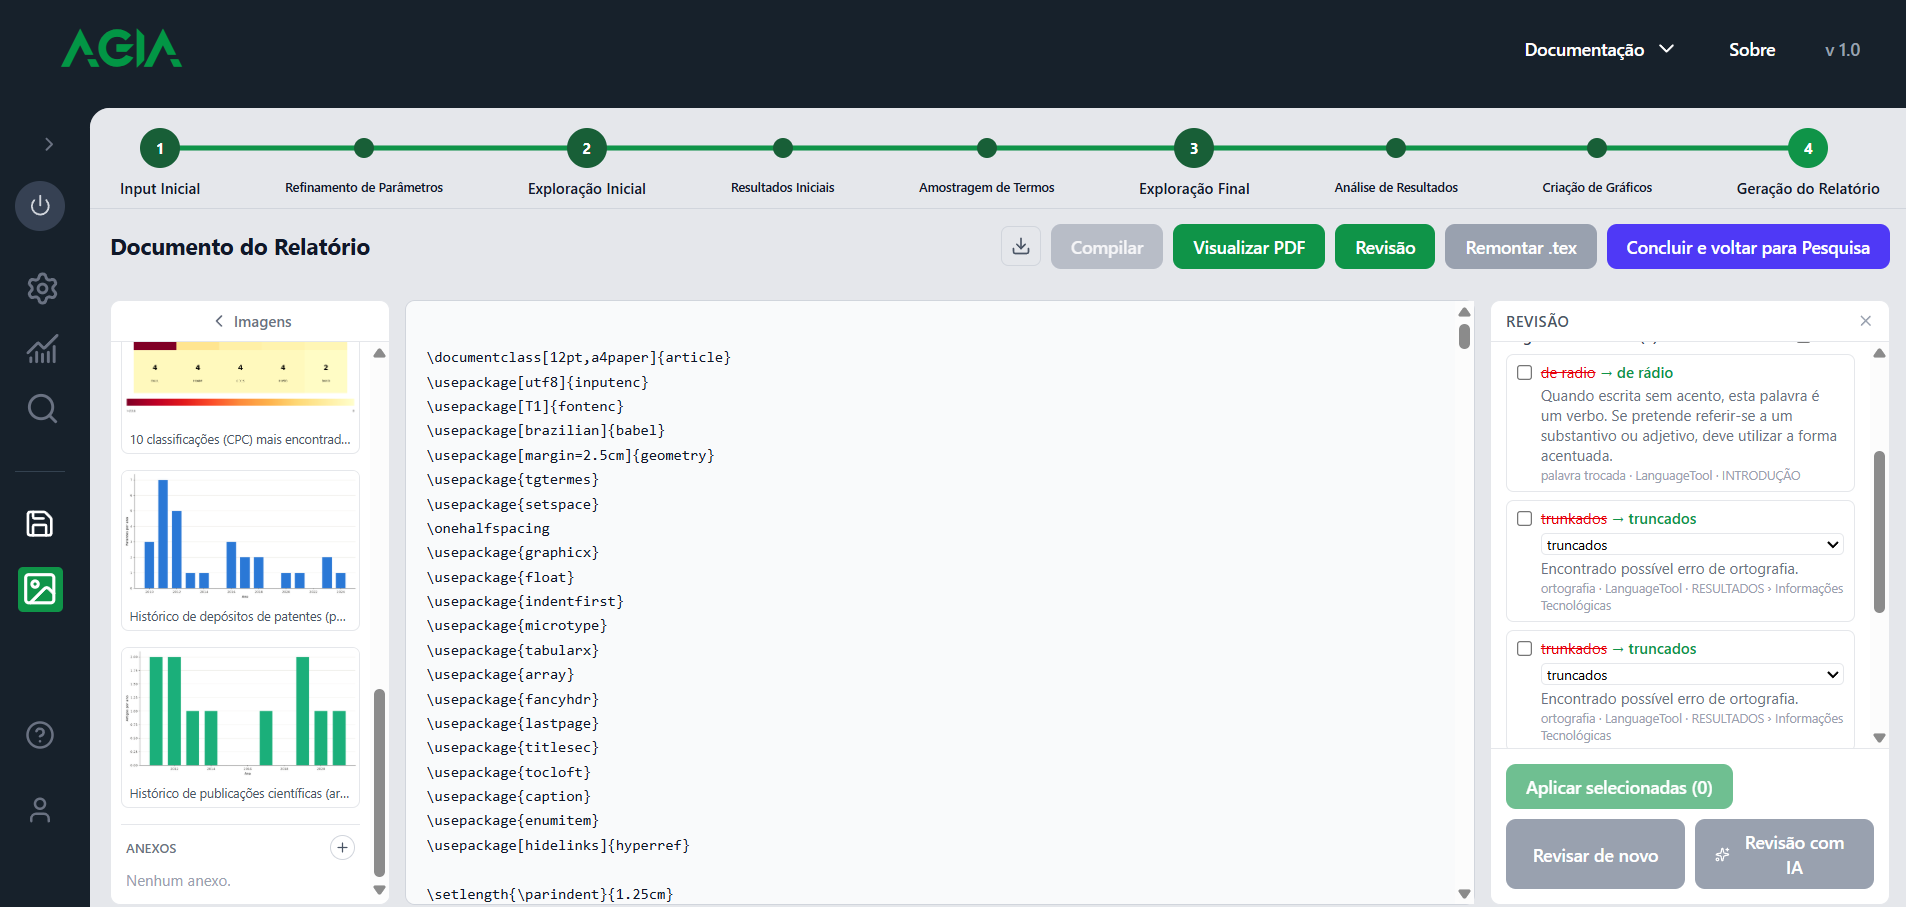
\includegraphics[keepaspectratio,alt={Painel de revisão com sugestões de correção, cada uma com caixa de seleção e explicação.}]{imagens/12-revisao.png}}
\caption{Painel de revisão com sugestões de correção, cada uma com caixa
de seleção e explicação.}
\end{figure}

\begin{itemize}
\tightlist
\item
  Cada sugestão mostra o trecho original riscado e a correção proposta,
  com uma explicação.
\item
  Marque as sugestões que quer aplicar e clique em \textbf{Aplicar
  selecionadas}. Nada é alterado sem a sua aprovação.
\item
  \textbf{Revisar de novo} refaz a análise do texto atual.
\item
  \textbf{Revisão com IA} pede uma revisão adicional feita pela IA.
\end{itemize}

Travas de segurança: uma sugestão só é aceita se o trecho existir
literalmente no texto e se a mudança for apenas de acento ou
concordância. Mudanças de tempo verbal, pontuação ou maiúsculas são
recusadas, assim como trocas de grafia.

\section{8.4 Compilação e pacotes
LaTeX}\label{compilauxe7uxe3o-e-pacotes-latex}

O PDF é gerado no servidor de compilação, \textbf{sem acesso à
internet}. Por isso, apenas os pacotes já instalados nesse servidor
podem ser usados.

\textbf{Já carregados pelo template} (podem ser usados no corpo do texto
sem \texttt{\textbackslash{}usepackage}):

\begin{itemize}
\tightlist
\item
  \texttt{graphicx} e \texttt{float} ---
  \texttt{\textbackslash{}includegraphics}, posicionamento
  \texttt{{[}H{]}};
\item
  \texttt{tabularx} e \texttt{array} --- tabelas com colunas \texttt{X},
  \texttt{p\{…\}}, \texttt{m\{…\}};
\item
  \texttt{enumitem} --- listas com rótulos customizados, ex.:
  \texttt{{[}label=}\allowbreak{}\texttt{\textbackslash{}alph*){]}};
\item
  \texttt{caption} --- \texttt{\textbackslash{}caption} e
  \texttt{\textbackslash{}captionof\{quadro\}\{…\}};
\item
  \texttt{hyperref} --- \texttt{\textbackslash{}ref},
  \texttt{\textbackslash{}pageref}, \texttt{\textbackslash{}url\{…\}},
  \texttt{\textbackslash{}href\{url\}\{texto\}};
\item
  \texttt{setspace} --- \texttt{\textbackslash{}singlespacing} e
  \texttt{\textbackslash{}onehalfspacing} (o documento usa espaçamento
  1,5);
\item
  \texttt{babel} em português --- hifenização e nomes como ``Figura'' e
  ``Sumário''.
\end{itemize}

Outros pacotes do preâmbulo (\texttt{geometry}, \texttt{fancyhdr},
\texttt{microtype}, \texttt{lastpage}, \texttt{titlesec},
\texttt{tocloft}, \texttt{indentfirst}, \texttt{tgtermes}) são
configurados pelo próprio template e não precisam ser alterados.

\textbf{Instalados, mas não carregados:} as coleções LaTeX recomendadas
e de fontes estão disponíveis. Se precisar de um deles, inclua o
\texttt{\textbackslash{}usepackage} no preâmbulo.

\textbf{Não disponíveis:} um \texttt{\textbackslash{}usepackage} de
pacote ausente interrompe a compilação com a mensagem ``File \ldots{}
.sty not found''. Exemplos: \texttt{multirow}, \texttt{makecell},
\texttt{siunitx}, \texttt{wrapfig}, \texttt{ulem}, \texttt{soul}.

Limitações do compilador:

\begin{itemize}
\tightlist
\item
  Usa \textbf{pdflatex}. \texttt{fontspec}, XeLaTeX e LuaLaTeX não
  funcionam.
\item
  Caracteres fora do alfabeto latino (chinês, japonês, cirílico etc.)
  não compilam.
\item
  A compilação tem limite de 120 segundos.
\end{itemize}

\textbf{Caracteres especiais:} o texto gerado pela IA e os campos do
formulário já saem escapados. Só o que você digita no editor precisa de
atenção: \texttt{\%}, \texttt{\&}, \texttt{\_} e \texttt{\#} devem ser
escritos como \texttt{\textbackslash{}\%}, \texttt{\textbackslash{}\&},
\texttt{\textbackslash{}\_} e \texttt{\textbackslash{}\#}.

\section{8.5 Figuras e referências}\label{figuras-e-referuxeancias}

\begin{itemize}
\tightlist
\item
  Figuras e quadros seguem o padrão REPTEC: título acima (``Figura N:''
  ou ``Quadro N:''), imagem centralizada e ``Fonte:'' abaixo.
\item
  Rótulos de figura usam o prefixo \texttt{fig:}, e os de quadro,
  \texttt{quadro:}.
\item
  Ao montar o documento, o sistema corrige ``Figura'' e ``Quadro'' antes
  de cada referência, com a concordância correta (a/o, da/do, na/no
  etc.).
\end{itemize}

\begin{center}\rule{0.5\linewidth}{0.5pt}\end{center}

\chapter{9. Salvar, voltar, continuar e
concluir}\label{salvar-voltar-continuar-e-concluir}

\section{9.1 Salvar progresso}\label{salvar-progresso}

O botão \textbf{Salvar Progresso} grava a sessão no servidor. Ele fica
disponível durante a prospecção, exceto enquanto a IA está processando
algo.

\begin{itemize}
\tightlist
\item
  A \textbf{primeira vez} que você salva, a sessão é criada.
\item
  Os salvamentos seguintes atualizam \textbf{a mesma sessão}.
\item
  O \textbf{tema é obrigatório} para salvar.
\end{itemize}

Até salvar, o que você preencheu fica apenas na tela aberta. Algumas
ações, como \textbf{Refinar parâmetros}, chamam a IA mesmo sem salvar.

\section{9.2 Voltar e avançar}\label{voltar-e-avanuxe7ar}

\textbf{Voltar} e \textbf{Avançar} não descartam o que já foi gerado.
Enquanto a sessão estiver aberta, o conteúdo fica guardado, e você volta
exatamente onde estava, sem chamar a IA de novo.

Cada etapa só oferece gerar de novo quando algo do qual ela depende
mudou.

\section{9.3 Continuar uma pesquisa}\label{continuar-uma-pesquisa}

Na tela de Busca, \textbf{Continuar pesquisa} reabre uma sessão pendente
na etapa em que ela foi salva, com documentos e termos restaurados, sem
consultar as bases de novo.

\section{9.4 Concluir a sessão}\label{concluir-a-sessuxe3o}

A sessão é \textbf{concluída} ao clicar em \textbf{Montar .tex} na
Geração do Relatório.

Depois disso, a pesquisa (queries, termos e buscas) \textbf{não pode
mais ser editada}. Só o texto do relatório continua editável.

\begin{center}\rule{0.5\linewidth}{0.5pt}\end{center}

\chapter{10. Tela de Busca}\label{tela-de-busca}

A tela \textbf{Sessões de Prospecção} lista as sessões salvas. Ela tem o
campo \textbf{Buscar por tema} (ex.: ``Drones'', ``IA em Saúde'') e três
filtros de status: \textbf{Todas}, \textbf{Pendentes} e
\textbf{Concluídas}.

\begin{figure}
\centering
\pandocbounded{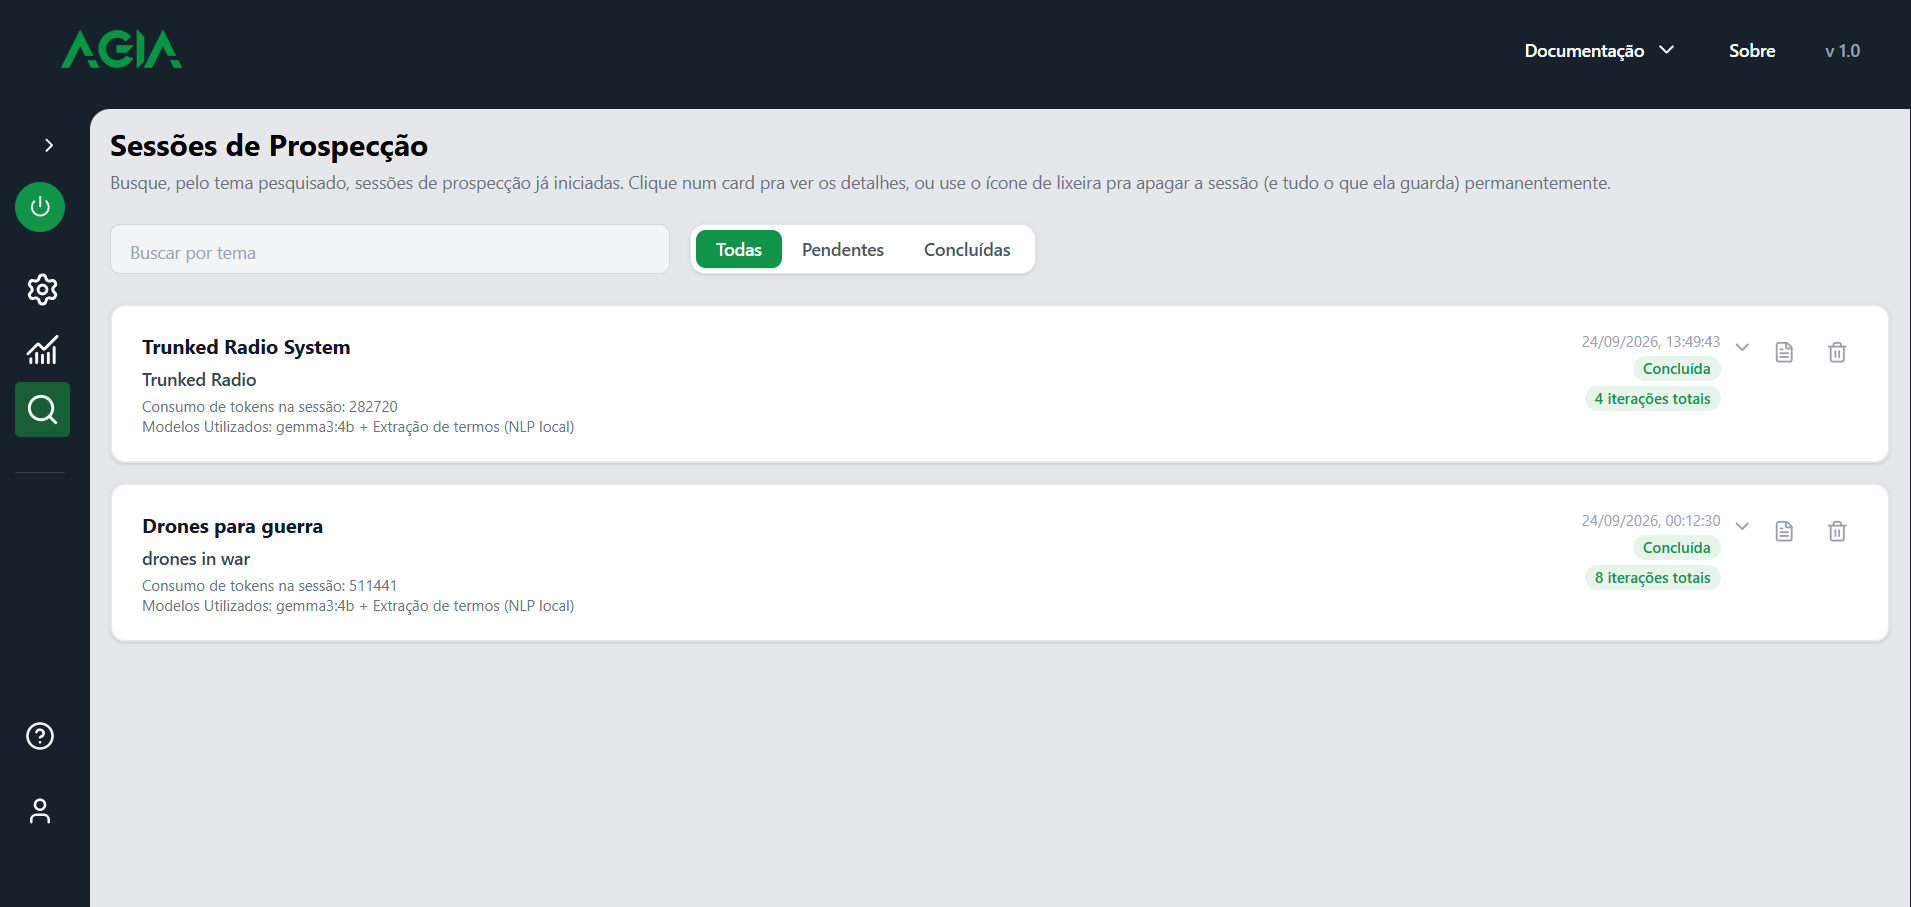
\includegraphics[keepaspectratio,alt={Lista de sessões salvas, com status, número de iterações, consumo de tokens e modelos usados.}]{imagens/01-sessoes.png}}
\caption{Lista de sessões salvas, com status, número de iterações,
consumo de tokens e modelos usados.}
\end{figure}

Cada cartão mostra:

\begin{itemize}
\tightlist
\item
  o \textbf{tema} da sessão e uma linha complementar;
\item
  o \textbf{consumo de tokens} da sessão;
\item
  os \textbf{modelos utilizados} (por exemplo, o modelo do Ollama e a
  extração de termos local);
\item
  a \textbf{data} de criação, o \textbf{status} (Concluída ou Pendente)
  e o \textbf{número de iterações} totais, ou seja, quantas rodadas de
  busca foram feitas.
\end{itemize}

Os ícones à direita de cada cartão:

\begin{itemize}
\tightlist
\item
  \textbf{seta} --- expande os detalhes da sessão;
\item
  \textbf{documento} --- abre o relatório da sessão (para sessões
  concluídas);
\item
  \textbf{lixeira} --- apaga a sessão e tudo o que ela guarda. Pede
  confirmação e \textbf{não é reversível}.
\end{itemize}

Além disso:

\begin{itemize}
\tightlist
\item
  \textbf{Continuar pesquisa} reabre uma sessão \textbf{pendente} na
  etapa em que foi salva.
\item
  \textbf{Ver Relatório} abre o editor de uma sessão \textbf{concluída}.
\end{itemize}

Sessões concluídas não podem mais ter a pesquisa alterada. Para uma nova
variante, crie outra prospecção.

\begin{center}\rule{0.5\linewidth}{0.5pt}\end{center}

\chapter{11. Tela de Estatísticas}\label{tela-de-estatuxedsticas}

A tela \textbf{Estatísticas das nossas prospecções} mostra o conjunto de
todas as sessões, com estes gráficos:

\begin{itemize}
\tightlist
\item
  \textbf{Sessões Concluídas x Pendentes} --- quantas sessões estão em
  cada status.
\item
  \textbf{Sessões em andamento x concluídas (últimos 30 dias)} ---
  evolução recente.
\item
  \textbf{Sessões por total de iterações} e \textbf{Prospecções por
  total de iterações} --- quantas rodadas de busca cada sessão precisou.
\item
  \textbf{Consumo médio de tokens} --- quanto de IA, em média, as
  sessões consumiram.
\end{itemize}

\begin{center}\rule{0.5\linewidth}{0.5pt}\end{center}

\chapter{12. Configurações (visão do
usuário)}\label{configurauxe7uxf5es-visuxe3o-do-usuuxe1rio}

A tela \textbf{Configurações} ajusta o comportamento do sistema. As
alterações são salvas automaticamente ao editar ou selecionar uma opção:
\textbf{não existe botão de salvar}.

Os parâmetros são agrupados em seis abas:

{\def\LTcaptype{none} % do not increment counter
\begin{longtable}[]{@{}
  >{\raggedright\arraybackslash}p{(\linewidth - 2\tabcolsep) * \real{0.3167}}
  >{\raggedright\arraybackslash}p{(\linewidth - 2\tabcolsep) * \real{0.6833}}@{}}
\toprule\noalign{}
\begin{minipage}[b]{\linewidth}\raggedright
Aba
\end{minipage} & \begin{minipage}[b]{\linewidth}\raggedright
O que controla
\end{minipage} \\
\midrule\noalign{}
\endhead
\bottomrule\noalign{}
\endlastfoot
\textbf{Inteligência Artificial} & Qual modelo de IA atende cada uso do
sistema. \\
\textbf{Busca} & Janela de anos da busca, tamanho das amostras e
credenciais das bases. \\
\textbf{Extração de Termos} & Pesos e critérios usados para escolher os
termos. \\
\textbf{Relevância \& Qualidade} & Corte de relevância dos resultados e
complexidade máxima das queries. \\
\textbf{Inferência Estatística} & Critérios de cobertura da amostra e de
estabilidade dos rankings. \\
\textbf{Geral} & Imagem de capa, idioma da revisão, modelo de embeddings
e tempo limite da IA local. \\
\end{longtable}
}

\section{12.1 Inteligência Artificial}\label{inteliguxeancia-artificial}

A seção \textbf{Qual IA cada chamada usa} define, para cada uso, qual
modelo responde:

\begin{figure}
\centering
\pandocbounded{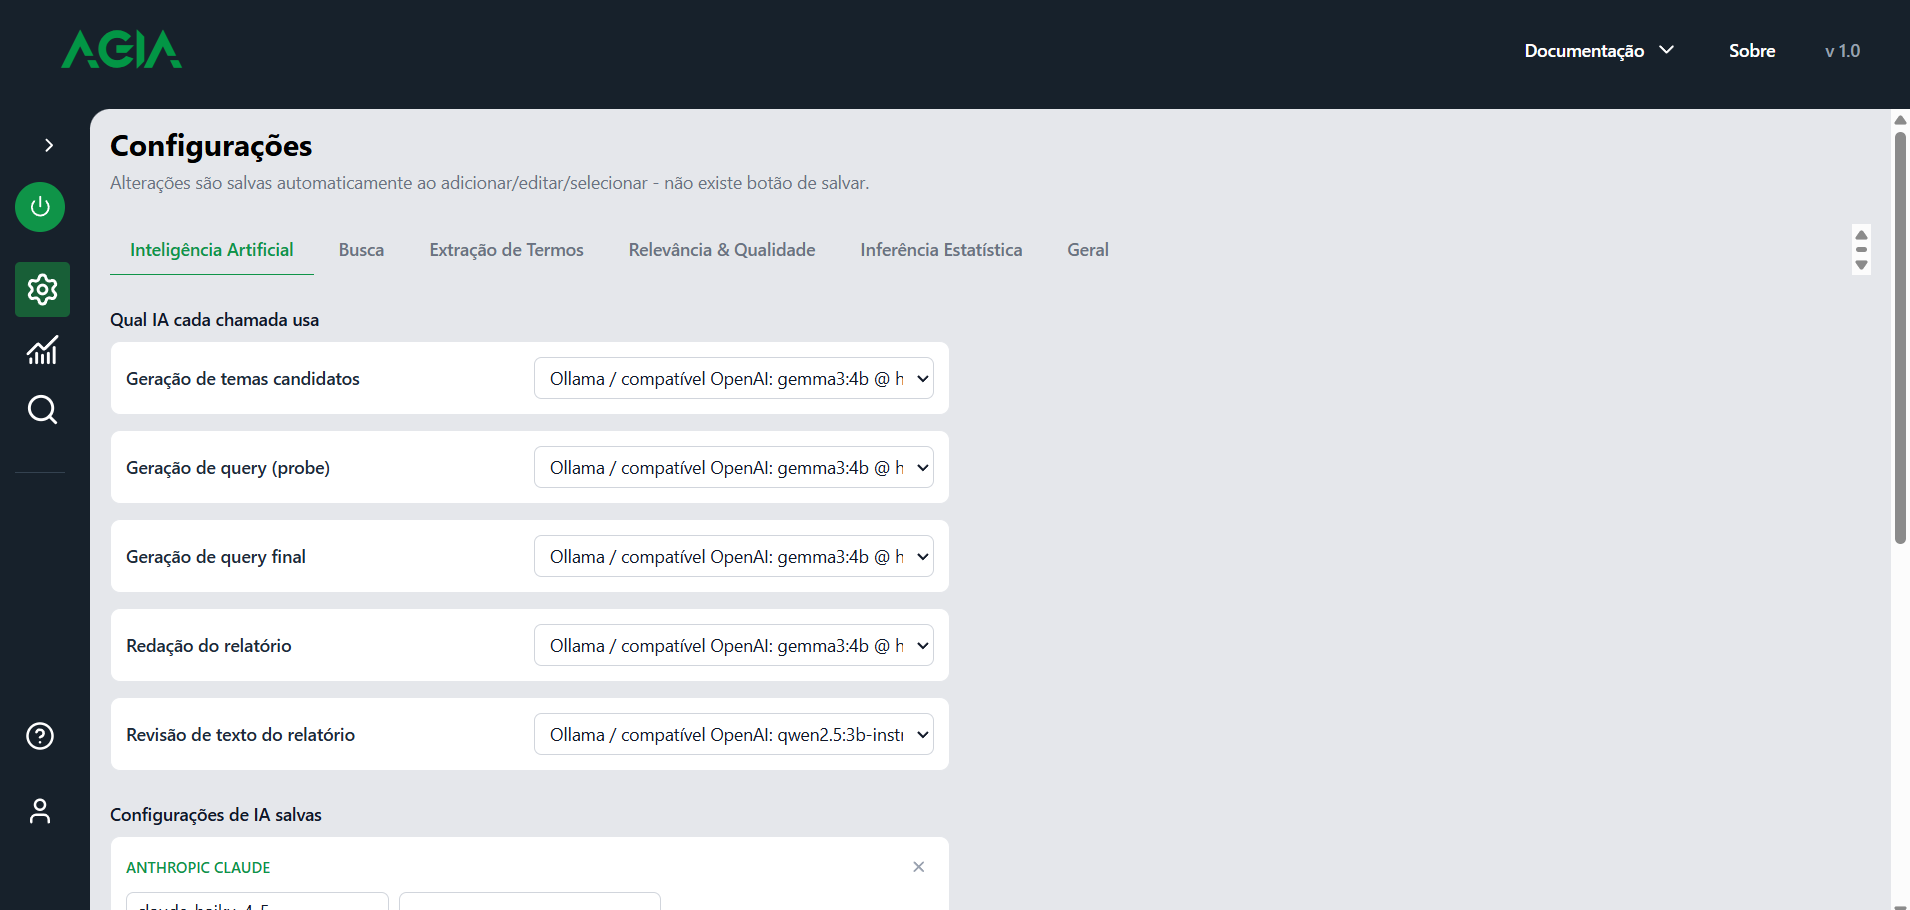
\includegraphics[keepaspectratio,alt={Configuração de IA: uma escolha de modelo para cada uso, e a lista de configurações de IA salvas.}]{imagens/13-config-ia.png}}
\caption{Configuração de IA: uma escolha de modelo para cada uso, e a
lista de configurações de IA salvas.}
\end{figure}

\begin{itemize}
\tightlist
\item
  \textbf{Geração de temas candidatos} --- as variações do tema, na
  etapa de refinamento.
\item
  \textbf{Geração de query (probe)} --- a query da busca exploratória.
\item
  \textbf{Geração de query final} --- a query da busca final.
\item
  \textbf{Redação do relatório} --- o texto das seções.
\item
  \textbf{Revisão de texto do relatório} --- as sugestões da revisão com
  IA.
\end{itemize}

Abaixo, \textbf{Configurações de IA salvas} lista os provedores
cadastrados, como o Ollama (que roda localmente) e o Anthropic Claude.
Você pode cadastrar novos provedores, e um mesmo provedor pode atender
vários usos.

\section{12.2 Geral}\label{geral}

\begin{figure}
\centering
\pandocbounded{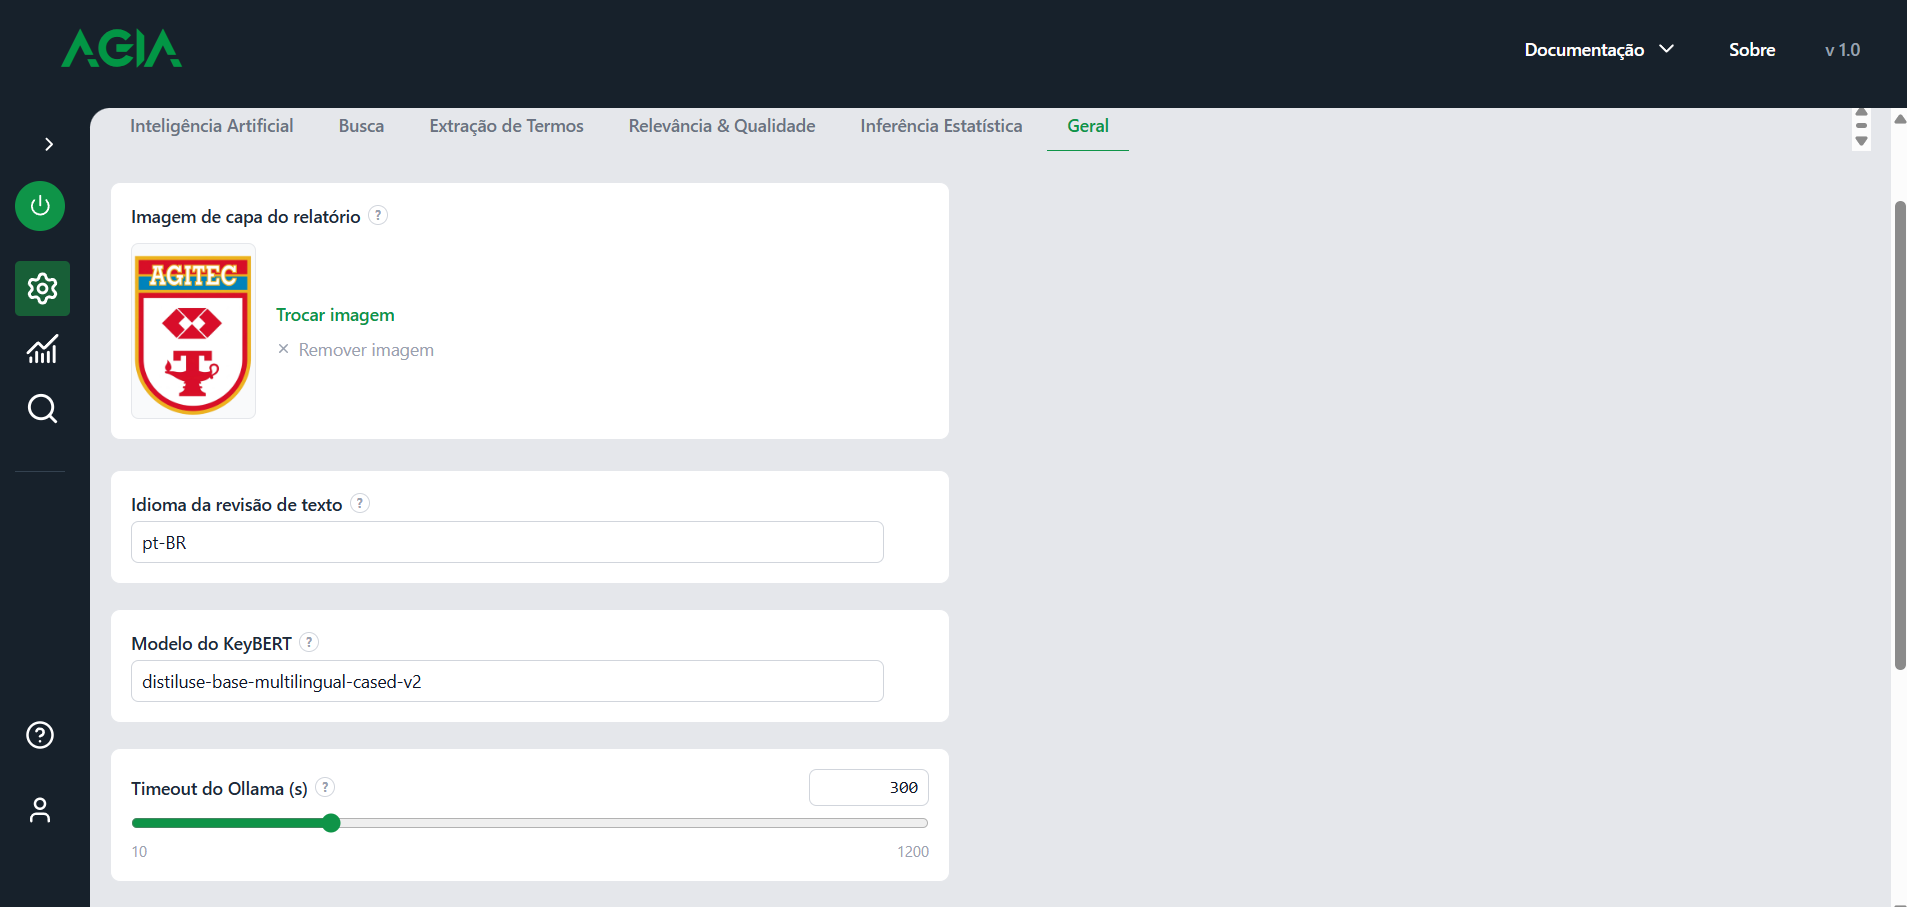
\includegraphics[keepaspectratio,alt={Configurações gerais: imagem de capa do relatório, idioma da revisão, modelo do KeyBERT e tempo limite do Ollama.}]{imagens/14-config-geral.png}}
\caption{Configurações gerais: imagem de capa do relatório, idioma da
revisão, modelo do KeyBERT e tempo limite do Ollama.}
\end{figure}

\begin{itemize}
\tightlist
\item
  \textbf{Imagem de capa do relatório} --- mostra a capa atual do
  REPTEC. \textbf{Trocar imagem} envia outra capa. Na versão atual, o
  botão de remoção é \textbf{Restaurar imagem padrão} e devolve a capa
  original do sistema (um brasão). A capa que você enviar nunca é
  sobrescrita pelo sistema ao reiniciar.
\item
  \textbf{Idioma da revisão de texto} --- idioma usado na revisão
  ortográfica (padrão pt-BR).
\item
  \textbf{Modelo do KeyBERT} --- modelo de embeddings da extração de
  termos e do RAG. Trocá-lo só tem efeito depois que o sistema for
  reiniciado.
\item
  \textbf{Timeout do Ollama (s)} --- tempo máximo de espera por uma
  resposta do modelo local. Modelos grandes ou em CPU precisam de mais
  tempo.
\end{itemize}

\begin{quote}
Alterar estas configurações afeta \textbf{todas} as prospecções
seguintes, não só a atual. Antes de mudar, anote o valor original.
\end{quote}

\begin{center}\rule{0.5\linewidth}{0.5pt}\end{center}

\chapter{13. Como o sistema funciona por
trás}\label{como-o-sistema-funciona-por-truxe1s}

Esta seção ajuda a entender os resultados. Não é necessária para usar o
sistema.

\section{13.1 Onde a IA entra}\label{onde-a-ia-entra}

A IA \textbf{não escreve a sintaxe final} da API de busca. Ela devolve
campos estruturados (termos de título, de resumo, de classificação
etc.), e um tradutor específico de cada base monta a expressão. Título e
resumo são combinados com OU; os demais campos, com E; o intervalo de
anos vira um filtro.

Campos editados manualmente são reconstruídos pelo mesmo tradutor,
\textbf{sem chamar a IA de novo}.

\section{13.2 Complexidade da query}\label{complexidade-da-query}

Queries longas e muito aninhadas quebram o processamento das bases ou
zeram a busca. Por isso, toda query gerada pela IA recebe uma
\textbf{nota de complexidade de 0 a 100} antes de ser enviada.

Se a nota passar do limite, a IA é chamada de novo pedindo uma versão
mais simples, com até três tentativas. Se nenhuma ficar abaixo do
limite, o sistema usa a menos complexa e mostra um aviso, em vez de
falhar.

\section{13.3 Busca exploratória}\label{busca-exploratuxf3ria}

Traz uma amostra pequena, \textbf{distribuída por ano} (para não se
concentrar nos documentos mais recentes). Documentos em outro idioma são
filtrados. Antes da extração de termos, um filtro de \textbf{relevância}
compara cada documento ao tema, e os que ficam abaixo do corte são
descartados.

\section{13.4 Extração de termos}\label{extrauxe7uxe3o-de-termos}

\begin{itemize}
\tightlist
\item
  Usa estatística (BM25F e RRF) e um modelo de embeddings, \textbf{sem
  IA generativa}.
\item
  Dá mais peso ao \textbf{título} do que ao resumo.
\item
  Prefere \textbf{frases de duas ou três palavras} a palavras isoladas,
  que costumam ser genéricas.
\item
  Descarta combinações com padrão gramatical ruim (por exemplo, advérbio
  seguido de verbo).
\end{itemize}

Por isso, o mesmo conjunto de documentos sempre gera os mesmos termos.

\section{13.5 Inferência
estatística}\label{inferuxeancia-estatuxedstica}

Ao criar os gráficos, o sistema verifica se a \textbf{amostra já cobre a
diversidade} real do campo:

\begin{itemize}
\tightlist
\item
  \textbf{Saturação (Chao1):} estima quantos depositantes, instituições,
  CPCs e áreas existem no total, a partir dos itens vistos uma ou duas
  vezes. Se a cobertura estimada for baixa, a amostra é considerada
  insuficiente.
\item
  \textbf{Estabilidade (bootstrap):} para cada item do top 10, mede em
  quantas reamostragens ele continua no top 10. Ranking instável indica
  amostra pequena para aquele agregado.
\end{itemize}

Depositantes e instituições têm \textbf{cauda longa} (muitos com um
único documento), por isso o ranking deles costuma ser menos estável.
Isso é esperado.

Se a amostra for insuficiente, o sistema repete a busca final pedindo
mais resultados, até saturar ou até o tempo máximo.

\section{13.6 Curva S e ciclo de vida}\label{curva-s-e-ciclo-de-vida}

\begin{itemize}
\tightlist
\item
  A curva logística (Fisher-Pry) é ajustada ao volume acumulado por ano.
  São necessários pelo menos \textbf{dois anos} com dados.
\item
  O \textbf{estágio do ciclo de vida} (Emergente, Crescimento,
  Maturidade ou Saturação) é calculado pelo sistema a partir dos pontos
  GP, MP e SP da curva. O texto do relatório recebe esse estágio pronto.
\item
  Um ajuste é considerado \textbf{não confiável} quando não passa em
  algum critério de qualidade: R² abaixo de 0,90, saturação alta com
  menos de 5 anos de dados ou taxa de crescimento implausível. Nesse
  caso, a curva é mostrada com aviso e sem a projeção.
\item
  Se o ajuste nem convergir (série ainda muito inicial), o gráfico é
  pulado.
\end{itemize}

\section{13.7 Gráficos e relatório}\label{gruxe1ficos-e-relatuxf3rio}

Os gráficos são gerados \textbf{a partir dos dados já coletados} da
busca final: nenhum gráfico dispara uma nova busca. Cada um é guardado e
recebe um resumo numérico, usado pelo texto para comentar a figura. Um
conjunto fixo de oito gráficos entra no relatório.

\begin{center}\rule{0.5\linewidth}{0.5pt}\end{center}

\chapter{14. Boas práticas e
limitações}\label{boas-pruxe1ticas-e-limitauxe7uxf5es}

\textbf{Boas práticas}

\begin{itemize}
\tightlist
\item
  \textbf{Comece amplo e afunile.} Use a exploração inicial para
  entender o campo antes de fixar a query final.
\item
  \textbf{Confira a amostra.} Se os resultados iniciais não batem com o
  tema, corrija antes de avançar.
\item
  \textbf{Escolha termos com critério.} Marque os termos que realmente
  definem o campo, não todos.
\item
  \textbf{Salve com frequência.} Use \textbf{Salvar Progresso} antes de
  fechar o navegador.
\item
  \textbf{Revise o texto da IA.} O sistema não substitui a leitura
  crítica. Confira dados, citações e conclusões antes de aprovar.
\item
  \textbf{Confira os metadados} antes de montar o .tex. Depois disso, só
  o texto é editável.
\end{itemize}

\textbf{Limitações}

\begin{itemize}
\tightlist
\item
  A busca depende das \textbf{bases externas}. Se elas estiverem lentas
  ou indisponíveis, os resultados podem sair incompletos.
\item
  \textbf{Credenciais de busca} são obrigatórias para obter resultados.
  Sem elas, as bases não retornam documentos.
\item
  \textbf{Textos da IA} podem não citar um documento que você esperava,
  porque só os trechos mais relevantes de cada seção entram no contexto.
\item
  \textbf{Compilação de PDF} não tem acesso à internet: pacotes LaTeX
  ausentes interrompem a compilação.
\item
  \textbf{Amostras pequenas} (poucos anos ou pouca variedade de
  documentos) geram análises menos confiáveis, sobretudo para
  depositantes e instituições. Os avisos de curva S e a inferência
  estatística ajudam a identificar esses casos.
\item
  \textbf{Sessões concluídas não são editáveis} na pesquisa.
\end{itemize}

\begin{center}\rule{0.5\linewidth}{0.5pt}\end{center}

\chapter{15. Perguntas frequentes}\label{perguntas-frequentes}

\textbf{Por que às vezes o botão mostra ``Avançar'' ou ``Ver
parâmetros'' em vez de ``Gerar Query'' ou ``Refinar parâmetros''?} O
sistema compara o que você preencheu agora com o que já foi gerado. Se
nada relevante mudou, reaproveita o resultado anterior, e o rótulo
indica que ele só vai avançar.

\textbf{Por que editar um campo em uma etapa anterior obriga a gerar
tudo de novo nas etapas seguintes?} Cada etapa depende do que foi
definido antes (tema, tema refinado, query escolhida). Ao mudar algo
para trás, o conteúdo gerado para frente deixa de corresponder à
entrada, e por isso é invalidado.

\textbf{Se eu clicar em Voltar, eu perco o que já tinha gerado?} Não.
Voltar e avançar restauram exatamente onde você estava, sem chamar a IA
de novo, a menos que algo em uma etapa anterior tenha mudado.

\textbf{Quando uma sessão passa a contar como concluída?} Ao clicar em
\textbf{Montar .tex} na Geração do Relatório. Até lá, \textbf{Salvar
Progresso} mantém a sessão pendente, para continuar depois pela tela de
Busca.

\textbf{Continuar uma pesquisa salva reabre onde eu parei?} Sim. Reabre
na etapa salva, com os documentos e termos restaurados do banco, sem
consultar as bases de novo.

\textbf{Por que não consigo sair da tela de prospecção sem confirmar
antes?} Enquanto a sessão está em andamento, o menu fica bloqueado e o
navegador avisa antes de fechar a aba, para evitar perder progresso não
salvo.

\textbf{Por que a Amostragem de Termos não tem um botão para gerar
outros termos?} Os termos são extraídos automaticamente, sem IA
generativa: os mesmos documentos sempre geram os mesmos termos. Para
obter termos diferentes, mude a query exploratória.

\textbf{Posso trocar o modelo do KeyBERT?} Sim, na aba Geral das
Configurações. A troca só vale depois de reiniciar o sistema.

\textbf{Por que meu \texttt{\textbackslash{}usepackage} faz a compilação
do PDF falhar?} O compilador roda sem internet e só tem os pacotes
instalados nele. Pacotes como \texttt{multirow}, \texttt{siunitx},
\texttt{wrapfig} ou \texttt{makecell} não estão disponíveis. Veja a
seção 8.4.

\textbf{Por que o texto da IA não cita um documento que eu esperava?} O
modelo só vê os trechos mais relevantes de cada seção, e o sistema
remove citações que não correspondam a esse contexto. Você pode citar o
documento manualmente no editor, ou ajustar ``Corte relativo do RAG'' e
``Top-K do RAG por seção'' na aba Geral e gerar a seção de novo.

\textbf{O que significa o aviso de ajuste pouco confiável na curva S?} O
ajuste logístico não passou em algum critério de qualidade. A curva
continua visível, sem a projeção, e deve ser lida com cautela. Buscas
com mais anos e mais documentos costumam resolver.

\textbf{Minhas edições no .tex são perdidas se eu gerar algo de novo?}
Só com \textbf{Remontar .tex}, que refaz o documento do zero e pede
confirmação antes. Compilar, revisar, inserir imagens ou baixar o .zip
nunca descartam edições.

\textbf{A busca voltou vazia. O que fazer?} Peça ao administrador para
confirmar que as credenciais de patente e de artigo estão preenchidas e
que o sistema foi reiniciado depois disso. Confira também se a query não
está complexa demais (medidor alto na Exploração Inicial).

\textbf{A IA demora muito para gerar.} Isso é mais comum quando o modelo
roda em CPU. Aguarde, ou peça ao administrador para verificar a
aceleração por placa de vídeo no servidor de IA.

\begin{center}\rule{0.5\linewidth}{0.5pt}\end{center}

\chapter{16. Glossário}\label{glossuxe1rio}

{\def\LTcaptype{none} % do not increment counter
\begin{longtable}[]{@{}
  >{\raggedright\arraybackslash}p{(\linewidth - 2\tabcolsep) * \real{0.2167}}
  >{\raggedright\arraybackslash}p{(\linewidth - 2\tabcolsep) * \real{0.7833}}@{}}
\toprule\noalign{}
\begin{minipage}[b]{\linewidth}\raggedright
Termo
\end{minipage} & \begin{minipage}[b]{\linewidth}\raggedright
Definição
\end{minipage} \\
\midrule\noalign{}
\endhead
\bottomrule\noalign{}
\endlastfoot
\textbf{Chao1} & Estimativa do número total de categorias (depositantes,
CPCs etc.) a partir dos itens vistos uma ou duas vezes. \\
\textbf{CPC} & Classificação Cooperativa de Patentes, usada para
classificar tecnologias. \\
\textbf{Curva S} & Gráfico da evolução cumulativa de documentos no
tempo, com modelo de ciclo de vida. \\
\textbf{Depositante} & Titular ou requerente de uma patente. \\
\textbf{Fisher-Pry} & Modelo logístico usado para ajustar a curva S. \\
\textbf{GP, MP, SP} & Pontos da curva S que marcam o início do
crescimento, o máximo e a saturação. \\
\textbf{IPC} & Classificação Internacional de Patentes. \\
\textbf{LanguageTool} & Ferramenta de revisão ortográfica e gramatical
usada pela revisão do editor. \\
\textbf{Lens} & Base de patentes e artigos, usada como alternativa às
demais. \\
\textbf{OPS} & Base de patentes do Escritório Europeu de Patentes
(EPO). \\
\textbf{Query} & Expressão de busca enviada às bases de dados. \\
\textbf{RAG} & Recuperação de trechos relevantes de uma base de
conhecimento, para embasar a geração de texto. \\
\textbf{REPTEC/AGITEC} & Modelo de relatório técnico adotado como
referência. \\
\textbf{Scopus} & Base de dados de artigos científicos. \\
\textbf{TermExtractor} & Componente que extrai os termos dos resultados,
sem IA generativa. \\
\textbf{Tokens} & Unidades de texto processadas pela IA; usadas para
medir o consumo de cada sessão. \\
\end{longtable}
}

\end{document}
